\documentclass[11pt,a4paper]{article}


\usepackage{natbib}
\bibliographystyle{plainnat}

% \usepackage[nottoc]{tocbibind}

\usepackage[english]{babel}
\usepackage{amsmath}
\usepackage{amssymb}
\usepackage{amsthm}
\newtheorem{theorem}{Theorem}[section]
\newtheorem{lemma}[theorem]{Lemma}
\newtheorem{corollary}[theorem]{Corollary}

\usepackage{newtxtext}
\usepackage[subscriptcorrection]{newtxmath}

\usepackage{bm}
\usepackage{bbold}
\usepackage{multicol}
\usepackage{graphicx}

\usepackage{tikz}
\usetikzlibrary{matrix,fit,backgrounds,positioning}
\usepackage{pgfplots}
\pgfplotsset{compat=1.18}

\usepackage[ruled,noend]{algorithm2e}

\usepackage{authblk}
\usepackage{lineno}
\usepackage{xcolor}
\usepackage{hyperref}
\usepackage[normalem]{ulem}

\DeclareMathOperator*{\argmax}{arg\,max}
\DeclareMathOperator*{\argmin}{arg\,min}

\makeatletter
\renewcommand{\algocf@captiontext}[2]{#1\algocf@typo. \AlCapFnt{}#2}
\renewcommand{\AlTitleFnt}[1]{#1\unskip}
\def\@algocf@capt@plain{top}
\renewcommand{\algocf@makecaption}[2]{%
  \addtolength{\hsize}{\algomargin}%
  \sbox\@tempboxa{\algocf@captiontext{#1}{#2}}%
  \ifdim\wd\@tempboxa >\hsize
    \hskip .5\algomargin%
    \parbox[t]{\hsize}{\algocf@captiontext{#1}{#2}}%
  \else
    \global\@minipagefalse%
    \hbox to\hsize{\box\@tempboxa}%
  \fi
  \addtolength{\hsize}{-\algomargin}%
}


\makeatother
%%% User-defined macros should be placed here, but keep them to a minimum.
\def\Bka{{\it Biometrika}}
\def\AIC{\textsc{aic}}
\def\T{{ \mathrm{\scriptscriptstyle T} }}
\def\v{{\varepsilon}}
\def\Clust{K}
\def\dataspace{\mathcal{D}}
\def\dglob{d_{\mathrm{\scriptscriptstyle glob}}}
\def\dloc{d_{\mathrm{\scriptscriptstyle loc}}}
\def\floor#1{\left\lfloor #1 \right\rfloor}
\def\globparam{\beta}
\def\iperm{l}
\def\istrat{h}
\def\Kmatch{K_{\text{match}}}
\def\Ksim{M}
\def\locparam{\mu}
\def\norm#1{\left\mid#1\right\rVert}
\def\Npart{N}
\def\Nperm{L}
\def\Npermstrat#1{L_{#1}}
\def\Nstrat{H}
\def\obsdata{\mathbf{y}}
\def\obsdataUn{y}
\def\param{\boldsymbol{\theta}}
\def\parprop{\boldsymbol{\theta}}
\def\parset{\Theta}
\def\proj{\varphi_{\obsdata}}
\def\remove#1{{\color{red} #1}}
\def\Rset{\mathbb{R}}
\def\simdata{\mathbf{z}}
\def\Varstrat{N}
\def\eps{\varepsilon}
\def\projsharp{{\varphi_{\mathbf{y}}}_{\sharp}}
\def\ca#1{\textcolor{red}{\textit{// CA: #1}}}
\def\al#1{\textcolor{purple}{\textit{// AL: #1}}}
\def\xian#1{\textcolor{orange}{\textit{// X: #1}}}
\def\rr#1{\textcolor{teal}{\textit{// RR: #1}}}

\newcommand{\new}[1]{\textcolor{blue}{#1}}
\newcommand{\old}[1]{\textcolor{red}{\sout{#1}}}
\title{Permutations Accelerate Approximate Bayesian Computation}

\author[1]{A. LUCIANO}
\author[1]{C. ANDRAL}
\author[1]{C. P. ROBERT}
\author[2]{R. J. RYDER}

\affil[1]{CEREMADE, UMR CNRS 7534, Université Paris Dauphine PSL\\
Place du Maréchal de Lattre de Tassigny, 75016 Paris, France\\
\texttt{luciano@ceremade.dauphine.fr}, \texttt{andral@ceremade.dauphine.fr}, \texttt{xian@ceremade.dauphine.fr}}

\affil[2]{Department of Mathematics, Imperial College London\\
South Kensington Campus, London SW7 2AZ, U.K.\\
\texttt{r.ryder@imperial.ac.uk}}

\date{}

\begin{document}

\maketitle
\linenumbers

\begin{abstract}
\input{sections/abstract}
\end{abstract}

\paragraph{Keywords.}
Approximate Bayesian Computation; Sequential Monte Carlo; Hierarchical models;
Permutation-based inference; Likelihood-free methods; Over-sampling;
Under-matching; Exchangeability.

\section*{Introduction}
\input{sections/0_intro}

\section{From ABC to permABC}
\label{secabc_to_permabc}

In this section, we will review the ABC framework and highlight its limitations within the hierarchical model framework. Subsequently, we will introduce our permutation-based method, permABC, which aims to address these limitations.

\subsection{Introduction to ABC}


The standard rejection ABC algorithm, often referred to as \emph{Vanilla ABC} (see Algorithm~\ref{alg:abc_vanilla}), proceeds by drawing parameters from the prior distribution, $\param \sim \pi(\cdot)$, and then simulating synthetic data from the likelihood, $\simdata \sim f(\cdot \mid \param)$. The pair $(\param, \simdata)$ is accepted if the summary statistics of the simulated data are sufficiently close to those of the observed data, that is, if $d\{\eta(\obsdata), \eta(\simdata)\} \leq \varepsilon$ for some tolerance level $\varepsilon > 0$ and some summary statistic $\eta$. This procedure yields samples from the approximate joint distribution $\pi_{\varepsilon}\{\param,\simdata \mid \eta(\obsdata)\}$; we marginalize out $\simdata$ to get the ABC posterior

\begin{equation}
    \label{eqabc}
    \begin{split}
        \pi_{\varepsilon}\{\param \mid \eta(\obsdata)\} &\propto
        \int_{\dataspace^\Clust} \pi_{\varepsilon}\{\param, \simdata \mid \eta(\obsdata)\} \, d\simdata \\
        &\propto \pi(\param) \int_{A_{\obsdata,\varepsilon}} f(\simdata \mid \param) \, d\simdata,
    \end{split}
\end{equation}
where $A_{\obsdata,\varepsilon} = \{\simdata \in \dataspace^\Clust \mid d\{\eta(\obsdata), \eta(\simdata)\} \leq \varepsilon\}$ denotes the acceptance region.

Combining an informative summary statistic $\eta$ with a small tolerance $\varepsilon$ typically leads to a good approximation of the true posterior distribution, so that $\pi_{\varepsilon}\{\param \mid \eta(\obsdata)\} \approx \pi(\param \mid \obsdata)$. This approximate posterior—often called a \emph{pseudo-posterior}—is obtained by replacing the true likelihood $f(\obsdata \mid \param)$ with the integral of the likelihood over the neighborhood $A_{\obsdata,\varepsilon}$ of the observed data, effectively using it as a surrogate for the intractable likelihood.

Throughout this work, we assume for clarity that the data are compared directly, i.e., $\eta = \mathrm{Id}$. Under this assumption, the acceptance region simplifies to the $\varepsilon$-ball $B_{\varepsilon}(\obsdata)$ centered at $\obsdata$ with respect to the distance $d$. Nonetheless, the proposed method naturally extends to the use of low-dimensional summary statistics.


In our numerical examples, we take $\dataspace = \mathbb R^n$ and use the distance $d(\cdot,\cdot)$ between two datasets in \( \dataspace^K \), each consisting of \( K \times n \) observations, defined as follows: 
\begin{equation}
    \label{eqdistance}
    d(\obsdata, \simdata)^2 = {\sum_{k=1}^K w_k^2 \| \obsdata_k - \simdata_k \|_2^2},
\end{equation}
where \( \| \cdot \|_2 \) denotes the Euclidean norm, and the weights \( w_k \) are used to control the relative influence of each compartment in the distance computation. The weight vector \( w_{1:K} \) can either be manually specified by the user or selected adaptively to prevent any single compartment from dominating the distance, as suggested by \citet{prangle2017adapting}.


This naive ABC algorithm faces several limitations, including poor scalability in the parameter space and an exponentially increasing computational cost due to the declining acceptance rate as \( \varepsilon \) decreases. In the context of the hierarchical model of Figure \ref{fig:hier}, the acceptance rate further diminishes as the number of compartments \( K \) increases. Simulating a dataset \( \simdata \) from the prior predictive distribution that matches all compartments of \( \obsdata \) within a small tolerance \( \varepsilon \) can be particularly challenging. 



\begin{algorithm}
\label{alg:abc_vanilla}
\caption{Vanilla Approximate Bayesian Computation}
\textbf{Input: }observed dataset $\obsdata$, number of iterations $N$ , threshold $\eps>0$, summary statistic $\eta$.\\
\textbf{Output: }a sample $(\param^{(1)}, \dots, \param^{(N)})$ from $\pi_\eps\{\cdot\mid\eta(\obsdata)\}$.\\

\BlankLine

\For{$i = 1,\dots, N$}{
    \Repeat{$d\{\eta(\simdata^{(i)}),\eta(\obsdata)\})\leq \eps$}{
        $\param^{(i)} \sim \pi(\cdot)$\;
        $\simdata^{(i)}\sim f(\cdot\mid\param^{(i)})$\;
        }
    }
\end{algorithm}


\subsection{Motivations of permABC}

A common approach in ABC to increase the acceptance rate is to exploit the exchangeability of the compartments by using a permutation-invariant summary statistic, such as the sorted vector. For instance, when we have a one-dimensional observation (or statistic) per compartment, $\obsdata \in \mathbb{R}^K$, it is natural to use the ordering $\eta(\obsdata) = \text{sort}(\obsdata)$ as a summary. \old{This reduces the effective complexity from $K!$ permutations to a canonical representation, thereby simplifying the comparison between datasets.}

Moreover, in the univariate case, sorting is known to minimize the distance over all permutations of simulated data. Specifically, $d\{\text{sort}(\obsdata), \text{sort}(\simdata)\} = \min_{\sigma \in \mathcal{S}_K} d(\obsdata, \simdata_{\sigma})$, where $\mathcal{S}_K$ denotes the set of all permutations of $\{1,\dots,K\}$. This property underlies several recent developments in ABC, including those based on optimal transport and Wasserstein distances \citep{bernton2019approximate}, where sorting plays a central role in defining distances between empirical distributions.

\new{This perspective is closely related in spirit to Wasserstein ABC (WABC) \citep{bernton2019approximate}, where inference is also based on a discrepancy between empirical distributions and is therefore intrinsically permutation-invariant at the data level. In WABC, however, the parameter of interest is global, and the method is designed for samples viewed as unordered point clouds. As a consequence, the issue of recovering compartment-specific local parameters is not addressed there. By contrast, our setting is hierarchical: while permutation invariance can be exploited to improve acceptance, inference ultimately concerns not only the global component \( \globparam \) but also the local parameters \( \locparam_{1:K} \), at least up to relabelling.}

\new{From a computational viewpoint, \citet{bernton2019approximate} also discuss several approximations to exact optimal transport in the multivariate case, including entropically regularized Sinkhorn divergences, Hilbert-curve sorting, and a greedy swapping refinement initialized from the Hilbert ordering. Using their notation, their sample size \(n\) corresponds here to the number \(K\) of compartments, whereas their observation dimension \(d_y\) corresponds to the dimension of each compartment-level observation. These approximations are particularly attractive when the number of points is very large, but the Hilbert-based approximation is reported to be accurate mainly for small observation dimension and to deteriorate as \(d_y\) grows. In our applications, \(K\) is only moderately large---with a limiting case around \(K=100\), which already corresponds to the scale at which WABC considers the number of data points---while the dimension of each compartment-level observation may be non-negligible. In this regime, approximate transport schemes can lose accuracy quickly, and solving the assignment problem exactly remains a practical and robust option.}

However, this elegant result no longer holds in the multivariate case. When each $\obsdata_k$ is a vector in $\mathbb{R}^n$ with $n > 1$, there is no natural way to define a deterministic and permutation-optimal ordering. \old{As a result, we cannot rely on sorting to minimize $d(\obsdata, \simdata_{\sigma})$ in general, and alternative strategies are needed as soon as the dimension is at least 2.} Instead, we are compelled to solve the optimization problem directly, which leads us to the following permABC acceptance criterion:
\begin{equation}
    \label{eqopti}
    \min_{\sigma \in \mathcal{S}_K} d(\obsdata, \simdata_{\sigma}) \leq \varepsilon.
\end{equation}

This condition can be interpreted as accepting if our simulated dataset $\simdata$ matches, up to a permutation, the observed dataset $\obsdata$, and it effectively enhances the acceptance rate by a factor of $K!$ when $\varepsilon$ is small. This optimization task can be formulated as a two-dimensional linear assignment problem, or equivalently a bipartite matching problem, and is efficiently solved using a modified Jonker--Volgenant algorithm \citep{jonker1987shortest}, with a computational complexity of $\mathcal{O}(K^3)$ \citep{crouseImplementing2DRectangular2016a}. While this reduces the combinatorial cost from $K!$ to polynomial time, the $\mathcal{O}(K^3)$ complexity remains substantial. Nevertheless, it makes problems with up to $K = 100$ compartments tractable in practice (see the real-world application in Section~\ref{sec:sir}).

However, this approach does not yield samples from the pseudo-posterior defined in \eqref{eqabc}, but rather from the following permutation-invariant version:
\begin{equation} 
    \label{eqpermabc_tilde}
    \begin{split}
        \Tilde \pi_{\varepsilon} (\param \mid \obsdata)  & \propto \int_{\dataspace^K} \Tilde \pi_{\varepsilon} (\param , \simdata \mid \obsdata) \, d\simdata \\
        & \propto \pi(\param) \int_{\Tilde A_{\obsdata,\varepsilon}} f(\simdata \mid \param) \, d\simdata,
    \end{split}
\end{equation}
where the acceptance region is defined as
\[
\tilde{A}_{\obsdata,\varepsilon} = \left\{\simdata \in \dataspace^K \,\middle|\, \min_{\sigma \in \mathcal{S}_K} d(\obsdata, \simdata_{\sigma}) \leq \varepsilon \right\} = \bigcup_{\sigma \in \mathcal{S}_K} B_{\varepsilon}(\obsdata_{\sigma}),
\]
with \( B_{\varepsilon}(\obsdata_{\sigma}) \) denoting the \( \varepsilon \)-ball centered at \( \obsdata_{\sigma} \) for the distance \( d \).

In this formulation, the likelihood \( f(\obsdata \mid \param) \) is approximated by its integral over a neighborhood of all permutations of the observed dataset:
\[
\int_{\tilde{A}_{\obsdata,\varepsilon}} f(\simdata \mid \param) \, d\simdata \approx \sum_{\sigma \in \mathcal{S}_K} f(\obsdata_{\sigma} \mid \param).
\]

Inference in this setting targets the global parameter \( \globparam \), but is only defined up to a permutation of the local components \( \locparam_{1:K} \), effectively yielding posterior samples of the form \( \Tilde{\param} = (\globparam, \{\locparam_1, \dots, \locparam_K\})\), where the local parameters are treated as an unordered set. \old{This formulation is particularly suitable when the local parameters are considered nuisance variables, as in many hierarchical modeling contexts.} We discuss below how to recover a pseudo-posterior of each $\mu_k$ if needed.

To our knowledge, this permutation-based version of ABC has not been formally studied in the literature. We therefore introduce a novel methodology, termed \emph{permABC}, which builds upon this idea while addressing its limitations. In particular, our method enables proper inference over the full parameter vector \( \param \), including the ordering of local components, even in regimes where \( K \) is large, and does so while preserving a high acceptance rate.

\subsection{The permABC algorithm}
\label{secpermabc_star}


Restoring identifiability among compartments is essential for enabling inference on the full parameter vector. One natural way to achieve this is by applying a suitable permutation to the accepted parameters, such that the simulated data are optimally aligned with the observed dataset. However, explicitly testing all \( K! \) permutations is computationally intractable.

Fortunately, whenever the acceptance condition \eqref{eqopti} is satisfied, there exists at least one permutation of the simulated dataset that meets the ABC criterion, namely the optimal one minimizing the distance. This permutation, denoted by \( \sigma^* = \argmin_{\sigma \in \mathcal{S}_K} d(\obsdata, \simdata_{\sigma}) \), provides a natural way to reorder the parameter vector.

In practice, the \emph{permABC} algorithm proceeds similarly to standard ABC: we sample \( \parprop \sim \pi(\cdot) \) and simulate data \( \simdata \sim f(\cdot \mid \parprop) \). If the minimum distance over all permutations satisfies the tolerance condition, we accept and return the pair \( (\parprop_{\sigma^*}, \simdata_{\sigma^*}) \). This induces a new pseudo-posterior distribution, denoted \( \pi_{\varepsilon}^*(\cdot, \cdot \mid \obsdata) \), which corresponds to the pushforward of the distribution \( \tilde{\pi}_\varepsilon \) defined in \eqref{eqpermabc_tilde} under the optimal alignment map \( \proj \):

\begin{equation}
\label{eqproj}
\pi^{*}_{\varepsilon}(\cdot, \cdot \mid \obsdata)
:= \projsharp \tilde{\pi}_{\varepsilon}(\cdot, \cdot \mid \obsdata)
\end{equation}
where
\[
\proj: (\param, \simdata) \mapsto (\param_{\sigma^*}, \simdata_{\sigma^*}).
\]
By construction, \( \proj \circ \proj = \proj \), so \( \proj \) acts as a projection. Moreover, its preimage satisfies \( \proj^{-1}(\{\param, \simdata\}) = \{(\param_{\sigma}, \simdata_{\sigma}) \mid \sigma \in \mathcal{S}_K\} \).

As a result, the projected pseudo-posterior satisfies:
\begin{equation*}
    \begin{split}
        \pi_{\varepsilon}^* (\param, \simdata \mid \obsdata) &  \propto \Tilde \pi_{\varepsilon} (\proj^{-1}(\{(\param, \simdata)\}) \mid \obsdata)\cdot \mathbb I_{\text{Im}(\proj)}(\param,\simdata)\\
        & \propto \sum_{\sigma} \Tilde \pi_{\varepsilon} (\param_{\sigma}, \simdata_{\sigma} \mid \obsdata)\cdot \mathbb I_{\text{Im}(\proj)}(\param,\simdata)\\
        % & \propto \sum_{\sigma} \pi(\param_{\sigma}) f(\simdata_{\sigma} \mid \param_{\sigma}) \mathbb{I}_{\tilde A_{\obsdata,\varepsilon}}(\simdata_{\sigma})\cdot \mathbb I_{\text{Im}(\proj)}(\param,\simdata)\\
        % & \propto \pi(\param) f(\simdata \mid \param) \mathbb{I}_{\tilde A_{\obsdata,\varepsilon}}(\simdata)\cdot \mathbb I_{\text{Im}(\proj)}(\param,\simdata)\\
        & \propto \tilde \pi_{\varepsilon}(\param, \simdata\mid \obsdata) \cdot \mathbb I_{\text{Im}(\proj)}(\param,\simdata).
    \end{split}
\end{equation*}


\noindent which enforces a constraint that accepted samples must lie in the image of the projection, i.e., must be optimally aligned with the observed data.

This additional constraint effectively restricts the integration domain to a subset of datasets that are optimally ordered with respect to \( \obsdata \). We define this constrained space as
\[
\dataspace_{\obsdata}^{*K} = \left\{ \simdata \in \dataspace^K \mid d(\obsdata, \simdata) = \min_{\sigma \in \mathcal{S}_K} d(\obsdata, \simdata_{\sigma}) \right\}.
\]
Consequently, the marginal pseudo-posterior can be expressed as:
\begin{equation}
\label{eqpermabc_star}
\pi_{\varepsilon}^*(\param \mid \obsdata) \propto \pi(\param) \int_{A_{\obsdata,\varepsilon}^*} f(\simdata \mid \param) \, d\simdata,
\end{equation}
where the new acceptance region is 
\[
A_{\obsdata,\varepsilon}^* = B_{\varepsilon}(\obsdata) \cap \dataspace_{\obsdata}^{*K}.
\]

The \emph{permABC} algorithm (see Algorithm~\ref{alg:permABC_star}) therefore defines a different approximation of the posterior distribution than classical ABC methods. In particular, it yields a different posterior approximation  \( \pi_{\varepsilon}^*(\cdot \mid \obsdata) \), which we shall compare to the vanilla ABC approximation \( \pi_{\varepsilon}(\cdot \mid \obsdata) \).


\begin{algorithm}
\SetKwInOut{Inputt}{Input}
\SetKwInOut{Outputt}{Output}
\caption{permABC Vanilla}\label{alg:permABC_star}
\textbf{Input: }observed dataset $\obsdata$, number of iterations $N$, threshold $\varepsilon>0$.\\
\textbf{Output: }a sample $(\param^{(1)}, \dots, \param^{(N)})$ from the pseudo-posterior distribution $\pi_{\varepsilon}^*(\cdot\mid \obsdata)$.\\

\BlankLine

\For{$i = 1,\dots, N$}{
    \Repeat{$d(\obsdata, \simdata_{\sigma^*}) \leq \eps$}{
        $\parprop \sim \pi(\cdot)$\;
        $\simdata \sim f(\cdot \mid \parprop)$\;
        $\sigma^* = \argmin_{\sigma \in \mathcal{S}_K} d(\obsdata, \simdata_{\sigma})$\;
    }
    $\param^{(i)} = \param'_{\sigma^*}\;$
}
\end{algorithm}

\subsection{Comparison with ABC}
\label{sec:comparison}

The permABC method introduced in the previous section (Algorithm~\ref{alg:permABC_star}) differs from standard ABC in a key aspect: instead of accepting all permutations that satisfy the ABC criterion, it retains only the optimal one—namely, the permutation that minimizes the discrepancy defined in Equation~\eqref{eqopti}. This choice, motivated by computational efficiency, alters the pseudo-posterior distribution by constraining the pseudo-data to lie within $\dataspace^{*K}_{\obsdata}$, as previously described.


In contrast, a variant equivalent to standard ABC would consist in uniformly sampling a permutation among those satisfying the ABC acceptance condition and appropriately reweighting the contribution of each accepted sample by the size of this set. However, enumerating this set incurs a prohibitive $K!$ computational complexity. In Appendix~\ref{sec:appendix_strat}, we propose a stratified sampling strategy—termed \emph{permABC-strat}—to efficiently estimate this cardinality and recover the standard pseudo-posterior.

To clarify the connection between permABC and standard ABC, we establish a sufficient condition under which both methods coincide. Specifically, we prove that when the tolerance $\varepsilon$ is small enough, the set of permutations satisfying the ABC criterion contains at most one element. We formalize this in the following lemma:

\begin{lemma}
\label{lempermABC_star}
Let $\obsdata \in \dataspace^K$ denote the observed dataset, and define the discrepancy function $d(\cdot, \cdot)$ as in Equation~\eqref{eqdistance}. Let
\[
\varepsilon^* := \min_{\sigma \neq \mathrm{Id}} \frac{1}{2} d(\obsdata, \obsdata_\sigma).
\]
Then for any $\varepsilon < \varepsilon^*$ and any simulated dataset $\simdata \in \mathbb{R}^{K \times n}$, at most one permutation satisfies the ABC criterion:
\[
\mathrm{Card} \left( \left\{ \sigma \in \mathcal{S}_K : d(\obsdata, \simdata_\sigma) \leq \varepsilon \right\} \right) \leq 1.
\]
\end{lemma}

The proofs of the preceding lemma, the following theorem, and the subsequent corollary are deferred to Appendix~\ref{appendix_proofs}. 

We make the assumption that no pair of compartments have the exact same observed data. This assumption implies that $\varepsilon^*>0$, and will in particular be verified almost surely for continuous data. It could be relaxed to take into account ties, but we do not consider such an extension here. Under this assumption, we can show that permABC and standard ABC agree for small enough $\varepsilon$, as formalized in the following results.

\begin{theorem}
\label{th:permABC_star}
Let $\pi^*_{\varepsilon}( \cdot \mid \obsdata)$ be the pseudo-posterior distribution resulting from the permABC algorithm, and $\pi_{\varepsilon}( \cdot \mid \obsdata)$ that obtained via standard ABC. Then, there exists $\varepsilon^*>0$ such that for all $\varepsilon < \varepsilon^*$, we have:
\[
\pi^*_{\varepsilon}( \cdot \mid \obsdata) = \pi_{\varepsilon}( \cdot \mid \obsdata).
\]
\end{theorem}

This equivalence ensures that permABC retains the same asymptotic behavior as standard ABC in the limit of vanishing tolerance. We summarize this in the following corollary:

\begin{corollary}
\label{col:permabc}
If the pseudo-posterior distribution $\pi_{\varepsilon}(\cdot \mid \obsdata)$ obtained by the ABC algorithm converges to the true posterior distribution as $\varepsilon \to 0$, then the pseudo-posterior distribution $\pi_{\varepsilon}^*(\cdot \mid \obsdata)$ obtained by the permABC algorithm also converges to the true posterior distribution as $\varepsilon \to 0$.
\end{corollary}

Thus, the efficiency gains provided by permABC come at no cost to theoretical consistency. For foundational results on ABC convergence, we refer to \citet{fearnhead2018abc}, who provides general conditions under which ABC approximations converge to the true posterior, along with error bounds.






\section{Sequential strategy with permutations}
\label{sec:sequential}
\subsection{Sequential ABC: state of the art and limitations}
\label{sec:abc_smc}
Rejection-based ABC methods, including the enhanced permABC, remain computationally expensive due to their reliance on the prior as a proposal distribution. 
Most methods in the ABC literature rely instead on more sophisticated proposals. A typical strategy is to propose from some distribution \( q(\param) \), then assign importance weights  of the form \( \pi(\param)/q(\param) \) to accepted samples to correct for the fact that they are not drawn from the prior \( \pi(\cdot) \). This produces weighted samples from the ABC pseudo-posterior \( \pi_\varepsilon(\param \mid \obsdata) \). 

Sequential importance sampling further improves efficiency by constructing a sequence of proposal distributions \( q_t(\cdot) \) over \( T \) iterations. Inspired by the Sequential Monte Carlo (SMC) framework \citep{delmoralSequentialMonteCarlo2006a}, several ABC-SMC algorithms have been developed \citep{sisson2007sequential,sissonCorrectionSissonSequential2009, toniApproximateBayesianComputation2008, beaumontAdaptiveApproximateBayesian2009b, delmoralAdaptiveSequentialMonte2012}, significantly improving convergence and computational performance.

These methods differ in their algorithmic design but follow the same principle: simulate from a sequence of intermediate ABC pseudo-posteriors \( \pi_{\varepsilon_0}, \dots, \pi_{\varepsilon_T} \), where the thresholds satisfy \( \varepsilon_0 = \infty > \varepsilon_1 > \dots > \varepsilon_T = \varepsilon \). Weights are updated iteratively, enabling efficient progression from the prior \( \pi_{\varepsilon_0}(\cdot \mid \obsdata) = \pi(\cdot) \) to the target pseudo-posterior \( \pi_\varepsilon(\cdot \mid \obsdata) \).

Here, we adopt the algorithm proposed by \citet{delmoralAdaptiveSequentialMonte2012}, widely used as a benchmark for ABC methods \citep{clarte2021componentwise}. This method combines a random walk proposal (see Section~\ref{sec:kernels}) with a Metropolis–Rosenbluth-Teller-Hastings (MRTH) acceptance step based on the ABC criterion and the MRTH ratio. 
%
A notable feature of this algorithm is the possibility to simulate \( M \) datasets \( \simdata^{(1)}, \dots, \simdata^{(M)} \) per parameter value \( \param \). 
While increasing \( M \) can reduce variance in the acceptance decision, setting \( M = 1 \) leads to better computational efficiency, as shown in practice by \citet{delmoralAdaptiveSequentialMonte2012} and in theory by \citet{bornn2017use}. 
With $M=1$, the importance weights become binary: they are equal to 1 if the particle is accepted (i.e., the distance is below \( \varepsilon \)) and 0 otherwise.

This simplification, however, induces a limitation. When weights are binary, the Effective Sample Size (ESS) reduces to the number of surviving particles. While ESS is commonly used to assess sample quality, it may not accurately reflect the true diversity of the sample, especially when the acceptance threshold is low. In such scenarios, repeated resampling steps tend to concentrate the population, leading to particle degeneracy. 
To address this issue, we propose using the \emph{unique particle rate} as a complementary diagnostic. This metric, defined as the proportion of distinct parameter values among the accepted particles, provides a more sensitive indicator of sample diversity. It offers a practical way to monitor degeneracy and evaluate the effective exploration of the pseudo-posterior during the sequential process. 
In contrast, the ABC-PMC algorithm originally introduced by \citet{sissonCorrectionSissonSequential2009} and later corrected by \citet{beaumontAdaptiveApproximateBayesian2009b} uses multinomial resampling, a practice discouraged in the SMC literature due to its inefficiency \citep{chopin2020introduction}.

In the following subsections, we propose three ways to accelerate ABC-SMC with permutations, based on three different strategies to define intermediate distributions.

\subsection{The permABC-SMC algorithm}

The adaptive SMC algorithm proposed by \citet{delmoralAdaptiveSequentialMonte2012} can be seamlessly extended to the permABC framework. By substituting the standard ABC acceptance criterion with the permutation-based criterion \eqref{eqopti}, we develop a sequential algorithm that targets the pseudo-posterior distribution \( \tilde{\pi}_\varepsilon(\param \mid \obsdata) \).

Upon reaching the stopping criterion or when \( \varepsilon_T = \varepsilon \), we apply the projection step \eqref{eqproj} to each particle in the final population \( \{(\param^{T,i}, \simdata^{T,i})\}_{i=1}^N \). This yields samples from the permuted pseudo-posterior \( \pi_\varepsilon^*(\param \mid \obsdata) \), effectively restoring identifiability among compartments.

It is essential to ensure that the proposal distributions \( q_t(\cdot) \) are adapted to the new acceptance criterion. We detail such kernels in Section~\ref{sec:kernels}, emphasizing their role in maintaining the efficiency of the sampling process under the permutation-based framework.

This approach, termed \emph{permABC-SMC}, facilitates a sequential transition from the prior to the permuted pseudo-posterior \( \pi^*_\varepsilon(\param \mid \obsdata) \). Thanks to proposal kernels tailored to the permutation-based selection rule, permABC-SMC enhances the exploration of the parameter space, particularly in high-dimensional settings where standard ABC methods may struggle.

The permABC-SMC approach is a natural way to extend permABC into a sequential method. It relies on intermediate distributions of the form $(\pi^*_{\varepsilon_t})_t$ which are similar to Over-Sequential ABC methods, and it already leads to substantial computational gains, as shown in Section \ref{sec:numeric}. Before we examine these practical results, we introduce two innovative sequences of intermediate distributions, with novel selection criteria which are only available because we rely on permutation-based matching.

\subsection{Over-Sampling}
\label{sec:permABC_OS}
The Over-Sampling strategy leverages the flexibility of the permABC framework to sample more efficiently from the target pseudo-posterior \( \pi_\varepsilon^*(\cdot \mid \obsdata) \) by simulating more compartments than are present in the observed data. Specifically, instead of generating \( K \) pseudo-compartments, we simulate \( M > K \) compartments: that is, we consider \( \simdata \in \dataspace^M \) while the observed data remain in \( \dataspace^K \). We then accept or reject based on the best simulated subset of size $K$.

To implement this strategy, we draw \( \param = (\globparam, \locparam_1, \dots, \locparam_M) \sim \pi(\cdot) \), simulate the corresponding data \( \simdata = (z_1, \dots, z_M) \sim f(\cdot \mid \param) \), and use the following acceptance condition:
\begin{equation}
    \label{eq:os}
    \min_{\sigma \in \mathcal{A}_K^M} d(\obsdata, \simdata_{\sigma}) \leq \varepsilon,
\end{equation}
where \( \mathcal{A}_K^M \) denotes the set of injections from \( \{1, \dots, K\} \) to \( \{1, \dots, M\} \), i.e., the set of partial \( K \)-permutations of \( \{1, \dots, M\} \). As in \eqref{eqopti}, this optimization problem can be solved efficiently using the same assignment algorithm with computational complexity \( \mathcal{O}(K^2 M) \) \citep{crouseImplementing2DRectangular2016a}.

We slightly abuse notation by denoting \( f \) the joint simulator over compartments, regardless of whether the number of compartments is \( K \) (observed) or \( M \) (simulated). This is justified since the simulator is defined componentwise via a common mechanism \( g \), applied independently to each compartment: formally, \( f(\simdata \mid \param) := \prod_{m=1}^M g(z_m \mid \globparam, \locparam_m) \).
 
Analogously to the case \( M = K \), this procedure defines a pseudo-posterior distribution \( \tilde{\pi}_\varepsilon^M(\cdot \mid \obsdata) \), and its projected version \( \pi_\varepsilon^{*M}(\cdot \mid \obsdata) \), which is obtained by applying the optimal partial permutation minimizing \eqref{eq:os} in a reasoning analogous to that of Section~\ref{secabc_to_permabc} (see Appendix~\ref{appendix_os} for details).

\new{More precisely, Over-Sampling can be viewed as a pushforward construction. Let \( \sigma^*=\sigma^*(\param,\simdata,\obsdata) \in \arg\min_{\sigma \in \mathcal{A}_K^M} d(\obsdata,\simdata_\sigma) \), using any measurable tie-breaking rule, and define the matching map}
\begin{equation}
    \Psi_{\obsdata}^{(M)} : (\param,\simdata) \longmapsto (\param^*,\simdata^*),
\end{equation}
\new{where}
\begin{equation}
    \simdata^* = \simdata_{\sigma^*} \in \dataspace^K,
    \qquad
    \param^* = \bigl(\globparam,\locparam_{\sigma^*(1)},\dots,\locparam_{\sigma^*(K)}\bigr).
\end{equation}
\new{Then the projected Over-Sampling distribution is exactly the pushforward}
\begin{equation}
    \pi_\varepsilon^{*M}(\cdot \mid \obsdata)
    =
    \bigl(\Psi_{\obsdata}^{(M)}\bigr)_\#
    \tilde{\pi}_\varepsilon^M(\cdot \mid \obsdata).
\end{equation}
\new{In other words, \( \tilde{\pi}_\varepsilon^M \) is the ABC law on the enlarged space \( (\globparam,\locparam_{1:M},\simdata_{1:M}) \), while \( \pi_\varepsilon^{*M} \) is obtained by projecting onto the \(K\) matched compartments and their associated local parameters.}

\old{Interestingly, the marginals in $\globparam$ and $\locparam$ exhibit contrasting behaviors as $M$ varies. When $M$ is large, the acceptance condition becomes easier to satisfy regardless of the value of $\varepsilon$, leading to a joint pseudo-posterior distribution close to the prior. Since the permutation only affects the local parameters, the marginal over $\globparam$ remains nearly unchanged, and therefore close to its prior distribution. In contrast, the marginal over the local parameters becomes more concentrated. This is because, when $M$ is large, the optimization in \eqref{eq:os} explores a wider set of potential matches, and the local parameters $\locparam_{1:K}$ corresponding to the best matching compartments are those that generate data most similar to $\obsdata$ under a given $\globparam$. As a result, these local components become tightly clustered around values that are locally optimal with respect to the matching criterion. As $M$ decreases toward $K$, this concentration fades, and the marginal over $\locparam$ gradually approaches the full permABC pseudo-posterior. This behavior is illustrated in Figure~\ref{fig:os}, and further discussed in Appendix~\ref{appendix_os}.}

\new{This pushforward representation also yields a clean asymptotic description of the regime \( M \to \infty \). Define}
\begin{equation}
    d_M(\obsdata,\simdata_{1:M})
    :=
    \min_{\sigma \in \mathcal{A}_K^M} d(\obsdata,\simdata_\sigma),
\end{equation}
\new{and, for fixed \( \globparam \), let}
\begin{equation}
    g_{\globparam}(z)
    :=
    \int g(z \mid \globparam,\mu)\,\pi(d\mu),
    \qquad
    S_{\globparam}
    :=
    \operatorname{supp}(g_{\globparam}).
\end{equation}
\new{We then introduce the support-based discrepancy}
\begin{equation}
    \delta_{\globparam}(\obsdata)
    :=
    \inf_{x_{1:K}\in S_{\globparam}^K} d(\obsdata,x_{1:K}).
\end{equation}
\new{Under mild regularity assumptions on \( d \), if \( Z_1,\dots,Z_M \mid \globparam \stackrel{\text{i.i.d.}}{\sim} g_{\globparam} \), then}
\begin{equation}
    d_M(\obsdata,Z_{1:M})
    \xrightarrow[M\to\infty]{a.s.}
    \delta_{\globparam}(\obsdata).
\end{equation}
\new{Hence, for every \( \varepsilon \) away from the boundary case \( \delta_{\globparam}(\obsdata)=\varepsilon \),}
\begin{equation}
    \mathbb{P}_{\globparam}\!\Bigl(
        d_M(\obsdata,Z_{1:M}) \le \varepsilon
    \Bigr)
    \xrightarrow[M\to\infty]{}
    \mathbf{1}\!\left\{
        \delta_{\globparam}(\obsdata)\le \varepsilon
    \right\}.
\end{equation}
\new{Therefore the marginal Over-Sampling pseudo-posterior on the global parameter satisfies}
\begin{equation}
    \tilde{\pi}_\varepsilon^M(\globparam \mid \obsdata)
    \propto
    \pi(\globparam)\,
    \mathbb{P}_{\globparam}\!\Bigl(
        d_M(\obsdata,Z_{1:M}) \le \varepsilon
    \Bigr)
    \xrightarrow[M\to\infty]{}
    \pi(\globparam)\,
    \mathbf{1}\!\left\{
        \delta_{\globparam}(\obsdata)\le \varepsilon
    \right\}.
\end{equation}
\new{In particular, if \( \delta_{\globparam}(\obsdata)=0 \) for every \( \globparam \) in the support of the prior, then for every \( \varepsilon>0 \),}
\begin{equation}
    \tilde{\pi}_\varepsilon^M(\globparam \mid \obsdata)
    \xrightarrow[M\to\infty]{}
    \pi(\globparam).
\end{equation}
\new{Thus, infinite Over-Sampling destroys all information on the global parameter: asymptotically, the ABC acceptance event no longer measures whether \( \globparam \) reproduces the observed compartments with the correct probability, but only whether the observed data lie in the support of the local marginal model. By contrast, the pushforward map \( \Psi_{\obsdata}^{(M)} \) still retains the \(K\) matched local parameters \( \locparam_{\sigma^*(1:K)} \), which explains why local marginals may become concentrated around good matching values even when the marginal in \( \globparam \) becomes nearly flat. As \( M \) decreases back to \( K \), this degeneracy disappears and the family \( \pi_\varepsilon^{*M} \) connects back continuously to the standard permABC pseudo-posterior. This behavior is illustrated in Figure~\ref{fig:os}, and further discussed in Appendix~\ref{appendix_os}.}

This new distribution family is particularly appealing, as it introduces a natural sequence of auxiliary distributions that converge to the target distribution \( \pi_\varepsilon^*(\cdot \mid \obsdata) \). We define a decreasing sequence \( M_0 > M_1 > \cdots > M_T = K \), keeping \( \varepsilon \) fixed, such that the acceptance condition \eqref{eq:os} becomes increasingly selective until it recovers the standard permABC criterion \eqref{eqopti} when \( M = K \). 
To navigate this sequence \( \left \{\tilde{\pi}_\varepsilon^{M_t}, t = 0, \dots, T \right\} \), we adapt the ABC-SMC framework of \citet{delmoralAdaptiveSequentialMonte2012}, as discussed in Section~\ref{sec:abc_smc}. At each stage, we apply the optimal partial permutation \( \sigma^* \) to each accepted particle to obtain a sample from \( \pi_\varepsilon^*(\cdot \mid \obsdata) \). This results in a new algorithm we call \emph{permABC-Over-Sampling (permABC-OS)}.

This method allows convergence to the target distribution in a reduced number of iterations. However, it also introduces several challenges that we now discuss. The first requirement for the success of the method is to initialize the algorithm with a sufficiently large and diverse population of accepted particles. To achieve this, one must choose $M_0$ and $\varepsilon$ in a coordinated manner. Specifically, since the minimum in \eqref{eq:os} decreases with $M$, a smaller value of $\varepsilon$ necessitates a larger $M_0$ in order to maintain a reasonable acceptance rate at the first iteration. In Appendix~\ref{appendix_os}, we propose a method to calibrate $\varepsilon$ as a function of $M_0$, thereby allowing users to set $M_0$ under a fixed simulation budget.

A second challenge attached to this method is the risk of extinction of the particle population during the sequential iterations. Specifically, when transitioning from population $t$ with $M_t$ compartments to population $t+1$ with $M_{t+1} < M_t$, the acceptance condition \eqref{eq:os} is evaluated on a reduced subset of simulated compartments. If compartments that previously matched observed ones are no longer considered, the particle may be rejected—even though it was previously accepted. To mitigate this, the sequence $M_t$ must be selected carefully. We provide a practical heuristic for this in Appendix~\ref{appendix_os}. 

Even under a careful design of the sequence $M_t$, a large portion of the population may be lost in this transition. To address this issue, we introduce a duplication mechanism whereby each particle is replicated across multiple random permutations. This increases the probability that at least one version of the particle survives the next acceptance test, without requiring additional simulations. The duplication strategy, along with heuristic guidelines for both selecting the sequence \( (M_t) \) and tuning \( \varepsilon \), is also detailed in Appendix~\ref{appendix_os}. 

\begin{figure}[htbp]
    \centering
    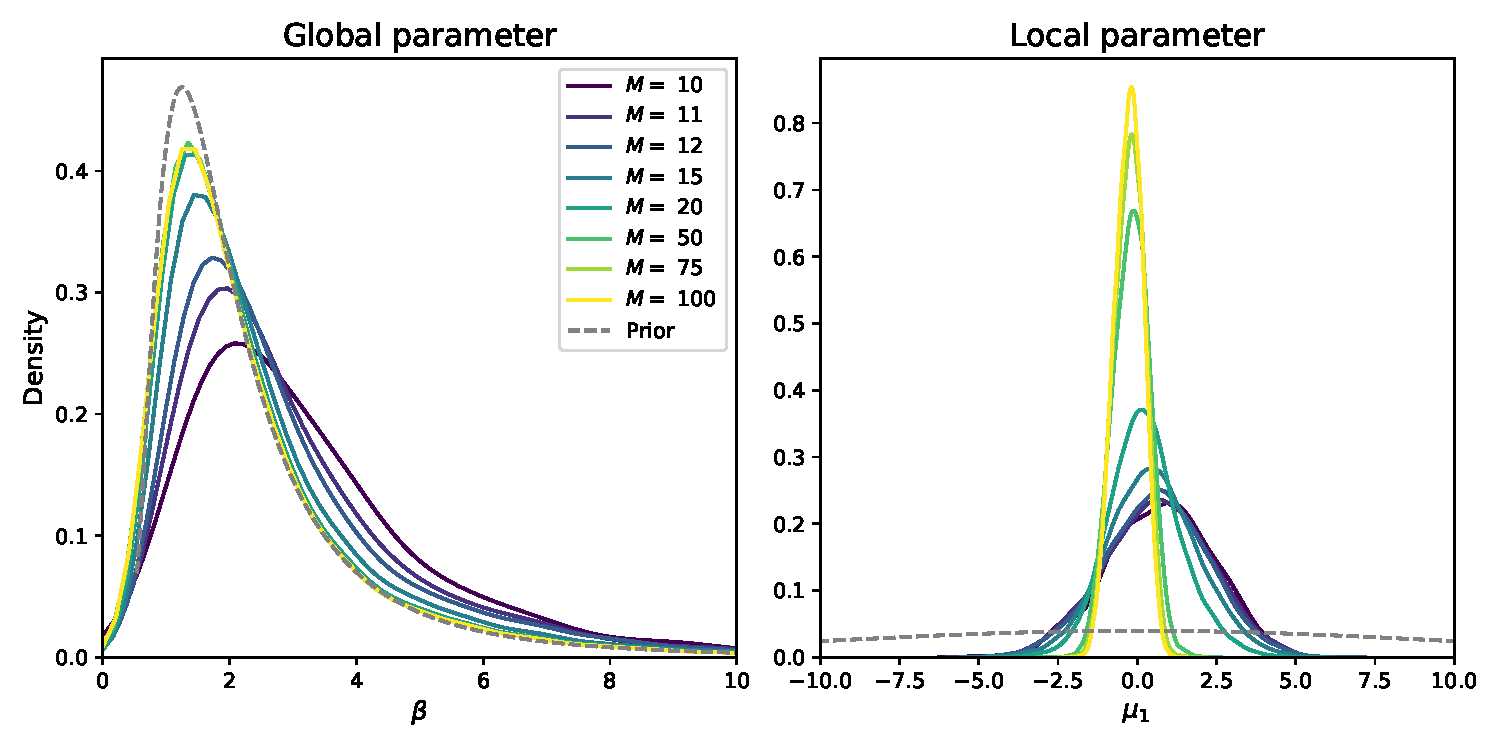
\includegraphics[scale=.5]{fig/fig2.pdf}
    \caption{Evolution of the pseudo-posterior \( \pi_\varepsilon^{*M} \) as \( M \) decreases from \( M_0 = 150 \) (yellow) to \( M_T = K = 10 \) (purple) for a Gaussian toy model.}
    \label{fig:os}
\end{figure}


\subsection{Under-Matching}
\label{sec:undermatching}
The under matching strategy—referred to as \emph{permABC-Under-Matching (permABC-UM)}—adopts a  perspective opposite to Over-Sampling. 
In this approach, we simulate synthetic data with the same number $K$ of compartments as the observed data; but at intermediate steps, we no longer require the simulated data to match all $K$ observed compartments. Instead, we simulate $K$ compartments but only require $L<K$ to match. The resulting acceptance criterion is defined as:
\begin{equation}
    \label{eqopti_um}
    \min_{\sigma \in \mathcal{A}_L^{K}, \tilde{\sigma} \in \mathcal{A}_L^{K}} d(\obsdata_{\tilde \sigma}, \simdata_{\sigma}) \leq \varepsilon,
\end{equation}
where \( \sigma \) and \( \tilde{\sigma} \) denote the sets of \( L \) selected compartments from the simulated and observed datasets, respectively. 


To solve this optimization problem efficiently, we extend the cost matrix by adding \( K - L \) dummy rows and \( K - L \) dummy columns with zero cost. These artificial entries ensure that \( K - L \) assignments are trivially matched, leaving the algorithm to find the best \( L \) true matches. This reduces the partial matching problem to a standard linear sum assignment problem on a square matrix of size \( (2K - L) \times (2K - L) \), which can be solved in \( \mathcal{O}\{(2K-L)^3\} \) time using classical algorithms \citep{crouseImplementing2DRectangular2016a}. 
 

This formulation allows for the algorithm to search over all possible \( L \)-sized subsets in both datasets, thereby relaxing the matching constraint and increasing flexibility in early iterations.

Although the distance \( d \) in Equation~\eqref{eqdistance} is defined for full datasets in \( \dataspace^K \), it naturally extends to subsets. In this context, given \( \sigma, \tilde \sigma \in \mathcal{A}_L^K \), the restricted distance is such that
\[
d(\obsdata_{\tilde \sigma}, \simdata_{\sigma})^2 = {\sum_{k=1}^L w_{\tilde \sigma(k)}^2 \| \obsdata_{\tilde \sigma(k)} - \simdata_{\sigma(k)} \|_2^2}.
\]
This formulation implies that compartments with higher weights have a greater impact on the acceptance condition, and are thus harder to match. This property can be exploited to prioritize compartments deemed more informative or robust, by appropriately adjusting the weights \( w_k \).

As in other variants of permABC, we employ a SMC scheme through a sequence of intermediate distributions \( \tilde{\pi}_\varepsilon^{L_t} \), corresponding to an increasing schedule \( L_0 < L_1 < \dots < L_T = K \). This gradual tightening of the matching criterion provides a smooth path toward the final target \( \pi^*_\varepsilon(\cdot \mid \obsdata) \), where all compartments are required to match.

Nevertheless, permABC-Under-Matching faces challenges similar to those of the Over-Sampling approach. In particular, it is crucial to select the initial tolerance \( \varepsilon \) appropriately, so as to ensure a sufficiently large and diverse first population. This requires calibrating \( \varepsilon \) as a function of \( L_0 \), the initial number of matched compartments, towards guaranteeing a high survival rate at the start of the algorithm.

Moreover, when the model is misspecified for even a single observed compartment, the final transition from \( L_{T-1} = K - 1 \) to \( L_T = K \) can lead to a sharp drop in the acceptance rate, resulting in severe particle degeneracy or even extinction. This makes the design of the sequence \( (L_t) \) and the level \( \varepsilon \) particularly critical for the success of the method. 
We show in Section \ref{sec:osum} that a well-designed under matching approach can increase performance in the presence of outliers.

These aspects are discussed in Appendix~\ref{appendix_um}, along with practical guidelines for choosing \( L_t \) and calibrating \( \varepsilon \) to avoid degeneracy. Situations where permABC-Under-Matching is especially advantageous, such as in the presence of outliers or structural model misspecification, are further investigated in Section~\ref{sec:osum}.

\subsection{Proposal Kernels for Permuted Inference}
\label{sec:kernels}


We recall that, by the abuse of notation introduced previously, we write \( \param_\sigma = (\globparam, \locparam_{\sigma(1)}, \dots, \locparam_{\sigma(K)}) \) to denote the parameter vector permuted by a given \( \sigma \in \mathcal{S}_K \), acting on the local components.


In the ABC-SMC framework of \citet{delmoralAdaptiveSequentialMonte2012}, the MCMC kernel \( K_t \) at iteration \( t \) uses a Gaussian random walk proposal \( q_t \) of the form:
\[
q_t(\cdot \mid \param) = \mathcal{N}\bigl\{\param, \operatorname{diag}\bigl(\tau_t^2\bigr)\bigr\},
\]
where \( \tau_t^2 \in \mathbb{R}^d \) is a vector of componentwise variances. These are typically defined as:
\[
\tau_t^2 = 2 \cdot \operatorname{var}\bigl\{\bigl(\param^{t-1,i}\bigr)_i\bigr\},
\]
i.e., twice the empirical variance across particles from the previous population. A Metropolis–Hastings correction step is then applied using the ABC acceptance criterion.

In the case of permABC-SMC, the exchangeability of the local parameters introduces label switching in the particle populations, which complicates the direct computation of componentwise variances. To resolve this, we first align the local parameters across particles using their optimal permutations \( \sigma_i^* \), and compute:
\[
\tau_t^2 = 2 \cdot \operatorname{var}\bigl\{\bigl(\param_{\sigma_i^*}^{t-1,i}\bigr)_i\bigr\}.
\]
This alignment restores parameter consistency across compartments, and allows us to maintain a diagonal Gaussian kernel with meaningful componentwise variances. The proposal kernel is then given by:
\[
q_t(\cdot \mid \param, \sigma) = \mathcal{N}\bigl[\param, \operatorname{diag}\bigl\{\sigma^{-1}(\tau_t^2)\bigr\}\bigr],
\]
where \( \sigma^{-1}(\tau_t^2) \) permutes the variance vector accordingly, so that each coordinate of \( \param \) is perturbed using the variance estimated in the appropriate reference frame.

In the case of \emph{Over-Sampling}, when the number of simulated compartments \( M \) exceeds the number of observed compartments \( K \), only a subset of the local parameters are matched to observations at each iteration. Let \( \mathcal{I} = \mathrm{Im}(\sigma^*) \subset \{1, \dots, M\} \) denote the indices of simulated compartments that are matched. For those indices, we reuse the corresponding variances from \( \tau_t^2 \) defined above. For the unmatched components \( k \notin \mathcal{I} \), we assign a default value:
\[
\tau_0^2 := \max_{k \in \mathcal{I}} \tau_t^2[k],
\]
which ensures exploration and numerical stability. This same default value \( \tau_0^2 \) is reused in the under-matching case below.





In the case of \emph{Under-Matching}, only a subset \( L_t < K \) of the observed compartments is matched at each iteration. For each particle \( i \), we define two injective mappings: \( \sigma_i \in \mathcal{A}_L^K \), which maps observed compartments to simulated compartments and \( \tilde{\sigma}_i \in \mathcal{A}_L^K \), which maps simulated compartments to observed ones.

The composition \( \tilde{\sigma}_i^{-1} \circ \sigma_i \) defines a partial permutation over observed indices, recovering the correspondence between an observed compartment \( k \in \{1, \dots, K\} \) and its matched simulated counterpart (when such a match exists for particle \( i \)). This matching allows us to construct a permutation-adjusted empirical variance over the population:
\[
\tau_t^2[k] = 2 \cdot \operatorname{Var} \left\{ \theta^{t-1,i}_{\tilde{\sigma}_i^{-1} \circ \sigma_i(k)} \right\}_i,
\]
defined only for those \( k \) that are matched in a sufficient number of particles. For unmatched coordinates, a default prior variance \( \tau_0^2 \) is used.


% In the case of under matching, only a subset \( L_t < K \) of observed compartments are matched at each iteration. Let \( \sigma \in \mathcal{A}_L^K \) and \( \tilde \sigma \in \mathcal{A}_L^K \) be the injections representing matches from observed to simulated compartments and vice versa. For each observed coordinate \( k \in \{1,\dots,K\} \), we define:
% \[
% \tau_t^2[k] = 2 \cdot \operatorname{var}\bigl\{\bigl(\theta_{\tilde \sigma_i^{-1} \circ \sigma_i(k)}^{t-1,i}\bigr)_i\bigr\},
% \]
% whenever the compartment \( k \) has been matched frequently enough across the population. If this condition is not met (e.g., in early iterations or due to sparse matching), we fallback to the default value \( \tau_t^2[k] = \tau_0^2 \).

% These variance assignment strategies allow us to construct robust and coherent Gaussian random walk proposals \( q_t \) for both global and local parameters across all three regimes: permABC-SMC, Over-Sampling, and Under-Matching.


These strategies ensure that Gaussian random walk proposals remain coherent and effective across all three regimes — standard permABC, Over-Sampling, and Under-Matching — by providing consistent scaling for both global and local parameters.



\section{Numerical experiments}
\label{sec:numeric}
\subsection{Comparison between ABC and permABC}
\label{sec:abc_vs_permabc}

As discussed in Section~\ref{sec:comparison}, permABC exhibits a different behavior from standard ABC. In particular, two regimes emerge depending on the value of the threshold \( \varepsilon \): when \( \varepsilon > \varepsilon^* \), permABC yields a different approximation of the posterior compared to ABC; whereas when \( \varepsilon \leq \varepsilon^* \), permABC coincides with standard ABC and thus inherits its convergence guarantees.
% \xian{La question étant quelle approximation est préférable ??}

To better illustrate the differences between the two approaches, we consider a simple toy model with no global parameter, defined as follows:
\[
\mu_k \sim \mathcal{U}(-2, 2), \quad \obsdata_k \sim \mathcal{U}(\mu_k - 1, \mu_k + 1), \quad k = 1, \dots, K,
\]
with \( K = 2 \), and a fixed observation \( y = (-1, 1)^\top \). 

Figure~\ref{fig:unif} highlights the two different regimes. When \( \varepsilon > \varepsilon^* \), permABC is concentrated in a region constrained by the order statistics, leading to a pseudo-posterior different from that of standard ABC. However, when the threshold satisfies \( \varepsilon \leq \varepsilon^* \), both methods recover the same pseudo-posterior. In this example, the critical value is \( \varepsilon^* = \sqrt{1/8}/2 \approx 0.177 \).


Note that, even in its vanilla form, permABC offers a significant gain in simulation efficiency. Since it effectively avoids redundant permutations during rejection, it reduces the required number of simulations by a factor of approximately \( K! \). In this simple example with \( K = 2 \), we achieve the same approximation quality (i.e., same \( \varepsilon < \varepsilon^* \)) using only half the number of simulations compared to standard ABC.

\begin{figure}[htbp]
    \centering
    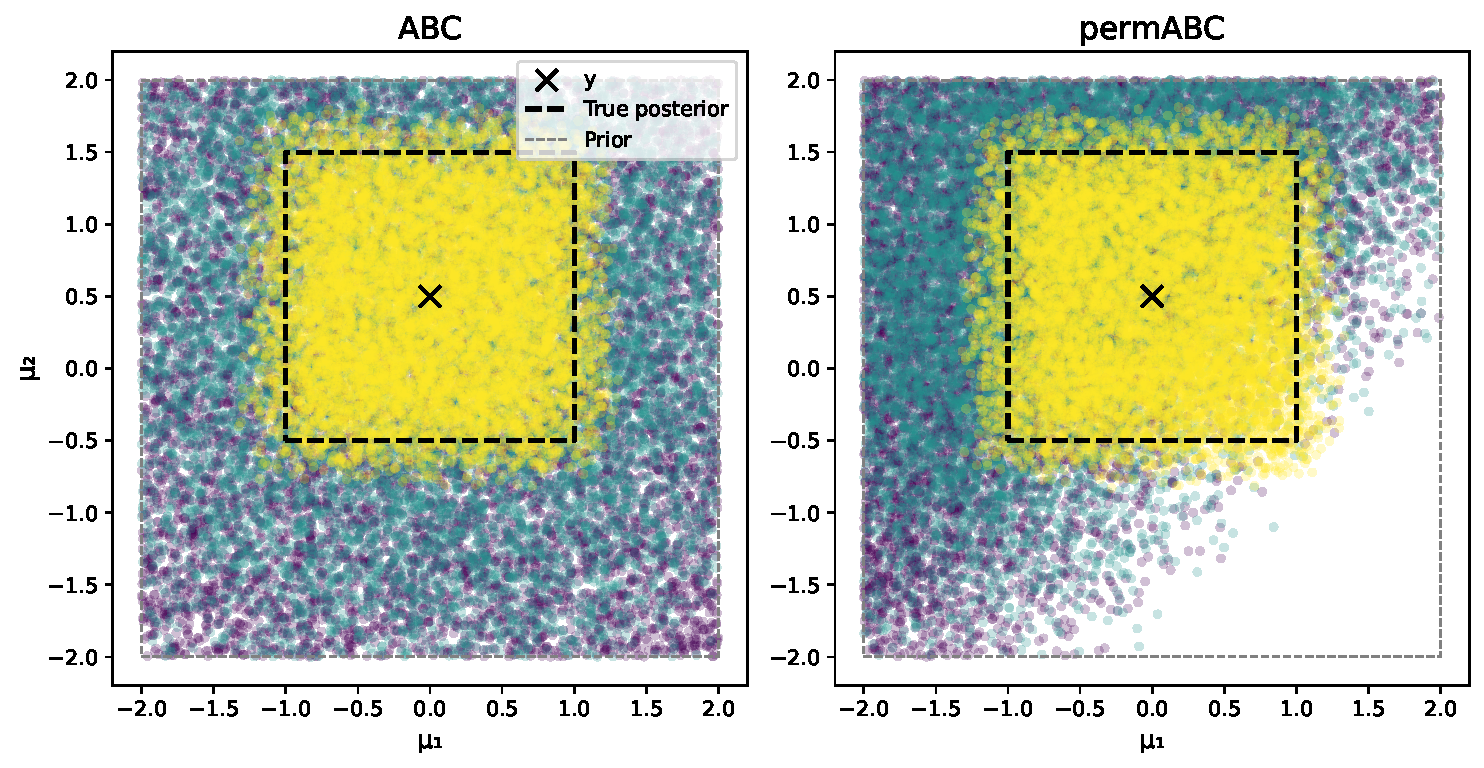
\includegraphics[scale=.5]{fig/fig3_seed_42.pdf}
    \caption{
        Comparison between standard ABC (left) and permABC (right) on the toy model of Section \ref{sec:abc_vs_permabc} with \( K = 2 \) and observation \( y = (-1, 1)^\top \). Each dot represents a sampled configuration \( \mu = (\mu_1, \mu_2) \), colored by the acceptance threshold used: purple for \( \varepsilon = \infty \), green for \( \varepsilon > \varepsilon^* \), and yellow for \( \varepsilon = \varepsilon^* \). The black cross denotes the observation \( y \), and the dashed box indicates the true posterior. While both methods recover the same posterior when \( \varepsilon < \varepsilon^* \), permABC avoids simulating permutations that are suboptimal at large \( \varepsilon \), resulting in a more concentrated distribution and improved efficiency. The two panels use the same computational budget.
    }
    \label{fig:unif}
\end{figure}
\subsection{Challenges of High-Dimensional ABC: A Gaussian Toy Model}
\label{sec:gaussian_toy}
We now consider a classical hierarchical model commonly used in the Bayesian literature:
\begin{equation*}
    \label{eqgauss}
    \beta \sim \mathrm{IG}(a,b), \quad \mu_k \sim \mathcal{N}(0, s^2), \quad \obsdata_{k} = (y_{1,k}, \dots, y_{n,k}) \overset{\text{i.i.d.}}{\sim} \mathcal{N}(\mu_k, \beta), \quad k = 1, \dots, K.
\end{equation*}

This simple yet representative model provides a convenient testbed to compare the various methods discussed in this paper, and to highlight the limitations of standard ABC approaches in high-dimensional settings. All ABC methods involve a fundamental trade-off between the number of simulations \( N \), the tolerance threshold \( \varepsilon \), and the effective number of accepted samples (or the number of unique particles in sequential schemes). A more efficient method achieves a lower value of \( \varepsilon \) for a given simulation budget \( N \) and fixed final sample size.

To enable fair comparison across methods, we adopt a consistent evaluation criterion: for each experiment, we report the value of \( \varepsilon \) achieved when the algorithm yields exactly 1,000 unique particles. In this setting, the number of simulations required to obtain a single unique accepted sample serves as a proxy for the effective sample size (ESS). This pseudo-ESS provides a normalized measure of sampling efficiency, which we use throughout our benchmarks.

Rejection-based algorithms such as vanilla ABC, as well as sequential variants like ABC-SMC and ABC-PMC, are known to scale poorly with the dimension of the parameter space, here indexed by the number of groups \( K \). As \( K \) increases, the acceptance rate drops sharply, resulting in a dramatic rise in computational cost. In contrast, the permutation-based acceptance rule introduced in permABC significantly improves the efficiency of both rejection and sequential samplers in high-dimensional regimes. The symmetry structure across local parameters \( \mu_1, \dots, \mu_K \) allows permABC to reduce redundant simulations and produce sharper approximations of the target pseudo-posterior.

Figure~\ref{fig:vanilla_vs_smc} illustrates this phenomenon: the methods proposed in this work achieve lower Monte Carlo error levels using fewer simulations, as reflected by smaller effective thresholds \( \varepsilon \). These gains become increasingly pronounced as \( K \) grows, confirming the advantage of permutation-based strategies in hierarchical or exchangeable models.

A complementary comparison in terms of wall-clock time — rather than simulation count — yields similar conclusions. This runtime-based analysis is provided in Appendix~\ref{sec:appendix_comparison}.


% \xian{¡No comprendo! L'axe des $x$ représente une efficacité décroissante ? Et c'est vraîment en $\log$-scale ??} 

\begin{figure}[htbp]
    \centering
    
\includegraphics[scale=.4]{fig/fig4_nsim_seed_42.pdf}
    \caption{
        Comparison of standard ABC methods and permutation-based variants in terms of achieved tolerance \( \varepsilon \) versus computational budget. The \( x \)-axis shows the number of simulations per 1,000 unique accepted particles (log-scale), and the \( y \)-axis represents the effective tolerance \( \varepsilon \) (log-scale). Lower values of \( \varepsilon \) correspond to more accurate approximations of the pseudo-posterior. Each curve represents a different algorithm. Permutation-based methods achieve substantially lower tolerance levels for the same simulation budget.
    }
    \label{fig:vanilla_vs_smc}
\end{figure}



\subsection{Failure cases of ABC-Gibbs}
\label{sec:abcgibbs_failure}

ABC-Gibbs methods \citep{clarte2021componentwise,rodrigues2020likelihood} have been designed to handle hierarchical models similar to those we consider. They are however less robust to model dependencies. We illustrate this with a modified hierarchical model designed to highlight the limitations of ABC-Gibbs:
\begin{equation*}
    \label{eqgauss_robin}
    \beta \sim \mathcal{N}(0, 10^2), \quad \mu_k \sim \mathcal{N}(0, 10^2), \quad \obsdata_k = (\obsdata_{1,k}, \dots, \obsdata_{n,k}) \overset{\text{i.i.d.}}{\sim} \mathcal{N}(\mu_k + \beta, 1), \quad k = 1, \dots, K.
\end{equation*}
This model is deliberately over-parameterized: it includes \( K+1 \) parameters for only \( K \) observations. Despite its simplicity, the posterior distribution exhibits a strong ridge structure due to the symmetry between local parameters \( \mu_k \) and the global parameter \( \beta \). This posterior can be reliably approximated using reference MCMC software such as PyMC. 
% \al{closed-form available? — to be computed.}

Figure~\ref{fig:perm_vs_gibbs} shows the two-dimensional marginal posterior over \( (\mu_1, \beta) \) obtained under a fixed simulation budget. While permABC-SMC provides a conservative and coherent approximation of the target posterior—as expected for an ABC method with global proposals—ABC-Gibbs produces a truncated approximation, failing to explore the full posterior support.

This discrepancy is rooted in the very structure of ABC-Gibbs. The algorithm proceeds by sequentially updating each parameter conditionally on the others using ABC rejection steps. In the presence of strong dependencies between parameters, as is the case here, the algorithm exhibits poor mixing: each marginal update is constrained by the current (possibly incorrect) values of the other parameters. As a result, the sampler explores a narrow region of the parameter space, failing to recover the full shape of the posterior.

These results underscore the limitations of coordinate-wise ABC approaches in models with strong local-global coupling. In contrast, permABC-based strategies, which jointly consider the full dataset and parameter configuration at each step, are more robust to such structural challenges.




\begin{figure}[htbp]
    \centering
    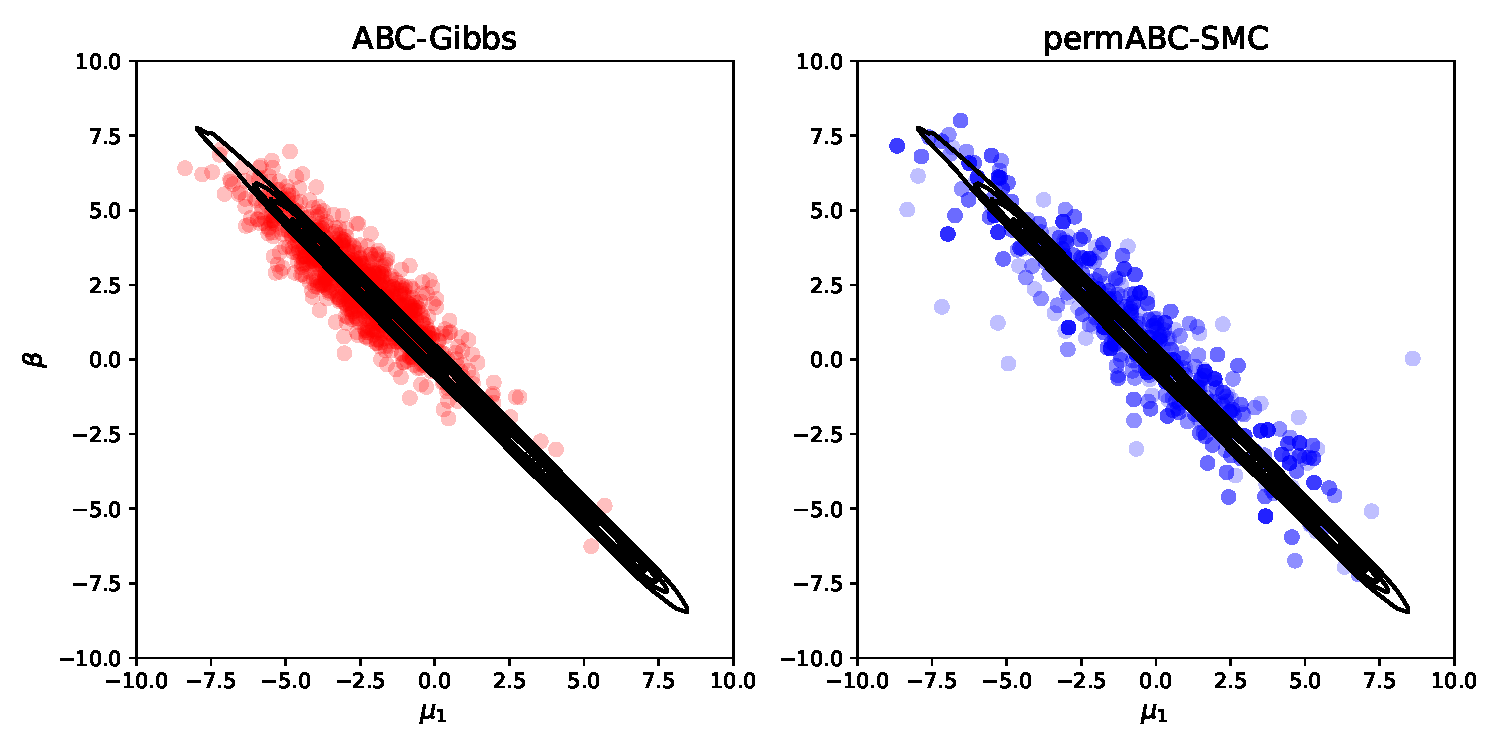
\includegraphics[scale=.5]{fig/fig5.pdf}
    \caption{
        Two-dimensional marginal posterior over \( (\mu_1, \beta) \) for the hierarchical model defined in Equation~\eqref{eqgauss_robin}, under a fixed simulation budget. The black ellipses represent level sets of the exact posterior distribution computed via MCMC (PyMC). Blue points correspond to samples produced by permABC-SMC, and red points to those produced by ABC-Gibbs. While permABC-SMC captures the full posterior geometry and respects the strong negative correlation between \( \mu_1 \) and \( \beta \), ABC-Gibbs fails to explore the posterior support. It becomes trapped along a narrow subset of the ridge, leading to a truncated and biased approximation. This illustrates the poor mixing behavior of coordinate-wise ABC samplers in the presence of strong global-local dependencies.
    }
    \label{fig:perm_vs_gibbs}
\end{figure}



\subsection{Discussion of the Over-Sampling and Under-Matching Approaches}
\label{sec:osum}

The Over-Sampling and Under-Matching strategies provide two complementary extensions of the permABC framework, each improving robustness and efficiency in different regimes of hierarchical inference under exchangeability.

We evaluate their performance on a Gaussian toy model with \( K = 20 \) compartments, among which 4 have local means \( \mu_k \) lying in the tails of the prior. This setup simulates a realistic scenario involving mild model misspecification or contamination by outliers. Figure~\ref{fig:osum} reports the total wall-clock time required to reach a given ABC threshold \( \varepsilon \), normalized by 1,000 unique accepted particles.

The Over-Sampling method (permABC-OS) achieves lower values of \( \varepsilon \) with shorter runtimes than standard permABC-SMC. While each iteration involves more expensive computations — due to larger assignment problems and duplicated particles (see Appendix~\ref{appendix_os}) — the faster convergence compensates for this cost, making the method highly effective even in the low-tolerance regime.

Under-Matching (permABC-UM) performs well in the intermediate-\( \varepsilon \) range. By relaxing the matching constraint to only \( L < K \) compartments, it allows rapid convergence while retaining robustness against model misspecification. However, as the algorithm transitions to full matching (\( L_t \to K \)), the acceptance condition tightens, often resulting in degeneracy of the particle population. Unlike in the OS strategy, this issue cannot be alleviated by duplication, and the method typically fails to reach very small values of \( \varepsilon \).

These contrasting behaviors suggest that combining the two strategies could yield additional benefits. One possibility is to begin inference with permABC-UM to quickly eliminate poorly fitting regions, then switch to permABC-SMC to refine toward smaller tolerances. More generally, hybrid schemes where \( L_t \) and \( M_t \) are jointly adapted — potentially alternating with changes in \( \varepsilon \) — offer a promising direction for future exploration.

A complementary figure reporting the number of simulations (instead of runtime) to reach the same target is provided in Appendix~\ref{sec:appendix_comparison}.

\begin{figure}[htbp]
    \centering
    
\includegraphics[scale=.4]{fig/fig6_time_seed_42.pdf}
    \caption{
        Comparison of standard ABC methods and permutation-based variants in terms of achieved tolerance \( \varepsilon \) versus wall-clock time. The \( x \)-axis shows the time required to obtain 1,000 unique accepted particles (log-scale), and the \( y \)-axis represents the effective tolerance \( \varepsilon \) (log-scale). Lower values of \( \varepsilon \) correspond to more accurate approximations of the pseudo-posterior. Each curve represents a different algorithm. Permutation-based methods — especially Over-Sampling and Under-Matching — achieve substantial efficiency gains in runtime.}
    \label{fig:osum}
\end{figure}






\subsection{Application to Real Data: The SIR Model}
\label{sec:sir}

In this final section, we illustrate the applicability of our methodology on real-world data by analysing the early spread of COVID-19 in France using publicly available hospitalization records from Santé publique France \citep{DataCovid}. The dataset provides daily hospital admissions at several geographic levels. We focus on mainland France (excluding overseas territories and Corsica), which yields 94 departmental time series.

To describe the epidemic dynamics, we use a classical Susceptible--Infectious--Recovered (SIR) model, defined through the latent system of ordinary differential equations
\begin{equation}
    \label{eqSIR}
    \begin{split}
        \frac{dS}{dt} &= -\delta \frac{SI}{N},\\
        \frac{dI}{dt} &= \delta \frac{SI}{N} - \nu I,\\
        \frac{dR}{dt} &= \nu I,
    \end{split}
\end{equation}
where \(S\), \(I\), and \(R\) denote the numbers of susceptible, infectious, and recovered individuals, respectively, \(N\) is the population size, and \(\delta\) and \(\nu\) are the transmission and recovery rates. The corresponding basic reproduction number is \(R_0 = \delta / \nu\).

Since the available data consist of hospital admissions rather than direct observations of the infectious compartment, the ODE system defines only a latent epidemic trajectory. To obtain simulated datasets, we combine the SIR dynamics with a stochastic observation model. Specifically, the transmission rate at each sub-daily time step is perturbed by a multiplicative log-normal noise:
\[
\delta_k^{(t)} = \delta_k \cdot \exp(\sigma \, \xi_k^{(t)}), \qquad \xi_k^{(t)} \overset{\text{i.i.d.}}{\sim} \mathcal{N}(0,1),
\]
with \(\sigma = 0.05\). This noise captures unmodelled day-to-day variability in transmission---due to reporting delays, local behavioural changes, or stochastic contact patterns---so that the simulated data entering the ABC distance are random even when the underlying SIR dynamics are deterministic. This distinction is important here, as ABC is applied to simulated observations rather than to the deterministic ODE solution itself.

To reduce confounding effects due to viral mutations and heterogeneous public-health responses, we restrict attention to the first epidemic wave, from March to July 2020. Over this period, the virus strain and the major national interventions were comparatively homogeneous across departments, making a simplified hierarchical formulation more reasonable.

Initial exploratory analyses (see Appendix~\ref{appendix_sir_validation}) suggest that the basic reproduction number \(R_0\) can be treated as a global parameter shared across departments. For each department \(k=1,\dots,94\), we introduce local parameters
\[
\locparam_k = \bigl(I_k(0), R_k(0), \nu_k\bigr),
\]
while setting \(\delta_k = R_0 \nu_k\). This yields a natural hierarchical structure with exchangeable local parameters and conditional independence across geographic compartments. When defining the distance between observed and simulated datasets (see \eqref{eqdistance}), the weights \(w_k\) may optionally be chosen proportional to the population size of each department in order to account for the different scales of the trajectories.

This application illustrates the type of high-dimensional hierarchical setting that motivated the development of permABC. With \(K=94\) compartments, three local parameters per department, and one global parameter \(R_0\), the resulting parameter space has dimension
\[
d = 3 \times 94 + 1 = 283.
\]
Such a setting is challenging for standard ABC methods, including sequential variants, because of the curse of dimensionality and the difficulty of efficiently exploring the space of local parameters. By contrast, permABC-SMC can exploit exchangeability across departments and can be combined with the independent-proposal Metropolis-within-Gibbs kernels of Section~\ref{sec:kernels} to perform inference at this scale.

Figure~\ref{fig_SIR_posterior} illustrates this point by comparing the posterior distributions of \(R_0\) obtained from aggregated national data and from the full collection of departmental trajectories. Using aggregated national data leads to flatter posterior distributions because substantial spatial information is lost. In contrast, the posterior distribution obtained with permABC-SMC from the 94 departmental time series is markedly more concentrated, reflecting the gain from jointly modelling shared global structure and department-specific heterogeneity. The inferred local heterogeneities are shown in the right panel of Figure~\ref{fig_SIR_posterior} and are also mapped geographically in Figure~\ref{fig_SIR_map}.

Despite these encouraging results, the SIR model remains a highly simplified description of epidemic dynamics and is inevitably misspecified when fitted to real hospitalization time series. In particular, the observation process linking infections to hospital admissions is only coarsely modelled, and many relevant mechanisms---such as reporting effects, delays, behavioural changes, and spatial interactions---are ignored. As a consequence, some posterior estimates of the local recovery rates \(\nu_k\) can take implausibly large values, which should be interpreted as compensating for model misspecification rather than as epidemiologically realistic estimates. This application should therefore be viewed primarily as a proof of scalability and practical relevance for permABC, rather than as a fully realistic epidemiological analysis.

\begin{figure}[htbp]
    \centering
    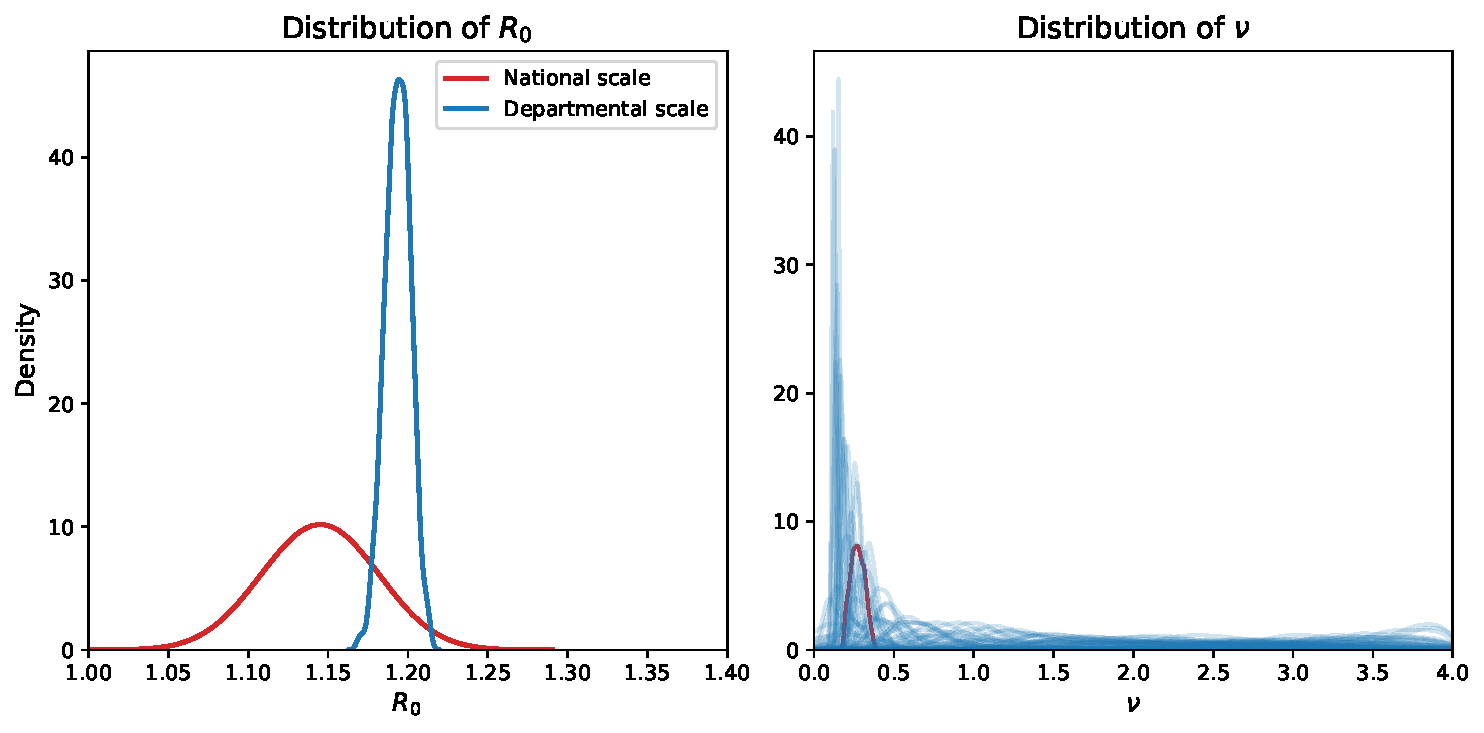
\includegraphics[scale=.5]{fig/fig7_posterior_comparison_seed_42.pdf}
    \caption{Posterior approximation for the global \(R_0\) parameter and the local recovery rates \(\nu_k\) in the hierarchical SIR model described in \eqref{eqSIR}, where \(R_0 = \delta / \nu\). The inference is performed using departmental-level data (\( K = 94 \), blue) or national-level aggregation (\(K = 1\), red).}
    \label{fig_SIR_posterior}
\end{figure}

\begin{figure}[htbp]
    \centering
    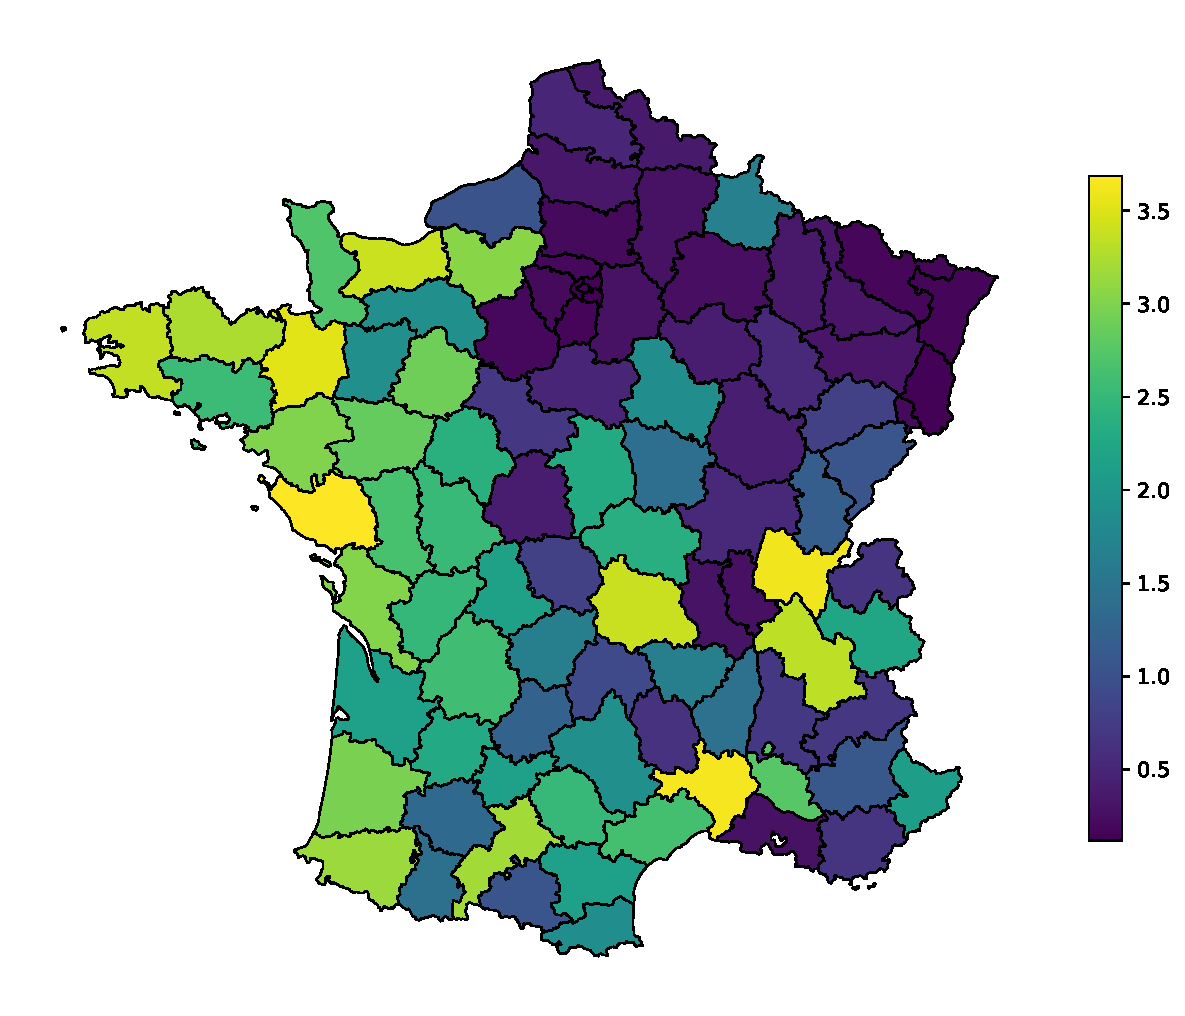
\includegraphics[scale=.5]{fig/fig8_map_departmental_seed_42.pdf}
    \caption{Map of the posterior mean estimates of the local recovery rate \(\nu_k\) for each department.}
    \label{fig_SIR_map}
\end{figure}


\section{Conclusion}
\input{sections/4_conclusion}


\bibliography{permABC}

\appendix
\section{Vanilla ABC Algorithm}
\label{appendix_vanilla_abc}

For completeness, we recall the standard rejection ABC algorithm \citep{marinApproximateBayesianComputational2012a}.

\begin{algorithm}
\label{alg:abc_vanilla}
\caption{Vanilla Approximate Bayesian Computation}
\textbf{Input: }observed dataset $\obsdata$, number of iterations $N$, threshold $\eps>0$, summary statistic $\eta$.\\
\textbf{Output: }a sample $(\param^{(1)}, \dots, \param^{(N)})$ from $\pi_\eps\{\cdot\mid\eta(\obsdata)\}$.\\

\BlankLine

\For{$i = 1,\dots, N$}{
    \Repeat{$d\{\eta(\simdata^{(i)}),\eta(\obsdata)\})\leq \eps$}{
        $\param^{(i)} \sim \pi(\cdot)$\;
        $\simdata^{(i)}\sim f(\cdot\mid\param^{(i)})$\;
        }
    }
\end{algorithm}

\section{Stratified version of permABC}
\label{sec:appendix_strat}

Even though permABC is equivalent to classical ABC in the small $\varepsilon$ regime, it differs outside of this regime because it integrates $\simdata$ into the constrained space $\dataspace_{\obsdata}^*$. Here, we propose a method called stratified permABC, which maintains the same acceptance rate but is exactly equivalent to ABC regardless of the value of $\varepsilon$.

In the stratified permABC algorithm, similar to the standard approach, we sample from the prior $\parprop \sim \pi(\cdot)$ and then sample data from the likelihood: $\simdata \sim f(\cdot \mid \parprop)$. Here, we consider the set of all permutations in the symmetric group $\mathcal{S}_K$, and determine the subset of acceptable permutations $\mathcal S_K^\varepsilon = { \sigma \in \mathcal S_K : d(\obsdata,\simdata_{\sigma}) \leq \varepsilon }$. The acceptance condition is then $\left | \mathcal S_K^\varepsilon \right | > 0$, which is equivalent to $\min_{\sigma \in \mathcal S_K} d(\obsdata,\simdata_{\sigma}) \leq \varepsilon$. We then accept the simulated $\parprop_{\sigma'}$, where $\sigma' \sim \mathcal U(\mathcal S_K^\varepsilon)$ with a weight proportional to $\lvert \mathcal S_K^\varepsilon \rvert$.

This methodology produces samples from the classical ABC pseudo-posterior distribution:
\begin{equation}
    \begin{split}
        \bar \pi_{\varepsilon} (\param \mid \obsdata) & \propto \pi(\param) \int_{A_{\obsdata,\varepsilon}} \frac{f(\simdata \mid \param)}{\lvert \mathcal S_K^\varepsilon \rvert} d\simdata \cdot \lvert \mathcal S_K^\varepsilon \rvert\\
        & \propto \pi_{\varepsilon} (\param \mid \obsdata)
    \end{split}
\end{equation}


However, this ABC scheme is impractical because it is too costly. Sampling $K!$ permutations is unfeasible. Thus, we can write this last quantity $\lvert \mathcal S_K^\varepsilon \rvert$ as $\mathbb{E}_{\sigma \sim \mathcal{U}(\mathcal{S}_K)}\left[\mathbb{I}_{A_{\obsdata,\varepsilon}}(\simdata_{\sigma})\right]$, which we will estimate by Monte Carlo. For small $\varepsilon$, a standard Monte Carlo simulation will have large variance: indeed, for most permutations $\sigma$, $d(\eta(\obsdata), \eta(\simdata_{\sigma})) > \varepsilon$, i.e., $\mathbb{I}_{A_{\obsdata,\varepsilon}}(\simdata_{\sigma})=0$. 

Instead, we resort to importance sampling. We write

\[\mathbb{E}_{\sigma \sim \mathcal{U}(\mathcal{S}_K)}\left[\mathbb{I}_{A_{\obsdata,\varepsilon}}(\simdata_{\sigma})\right] = 
\mathbb{E}_{\sigma \sim \rho}\left[\frac{\mathbb{I}_{A_{\obsdata,\varepsilon}}(\simdata_{\sigma})}{K!\rho(\sigma)}\right]\]

To do this, we sample $\sigma_{\iperm} \sim \rho(\sigma)$ for $\iperm=1,\dots, L$ and replace the weights $\lvert \mathcal S_K^\varepsilon \rvert$ by the following importance sampling estimator: $\frac{1}{L}\sum_{l=1}^L \frac{\mathbb{I}_{A_{\obsdata,\varepsilon}}(\simdata_{\sigma_{\iperm}})}{\rho(\sigma_{\iperm})}$. 

% We obtain the approximation:
% \begin{equation}
%     \pi_{\varepsilon} (\param \mid \obsdata)  \approx \pi(\param) \int   f(\simdata \mid \param) \sum_{\iperm=1}^L \frac{\mathbb{I}_{A_{\obsdata,\varepsilon}}(\simdata_{\sigma_{\iperm}})}{\rho(\sigma_{\iperm})} d\simdata
% \end{equation}


We now look for a good proposal distribution $\rho$ over $\mathcal{S}_K$.

\subsection{Simulating Non-uniform Permutations}
\label{secperm}

A good proposal $\pi$ will have support all of the symmetric group $\mathcal{S}_K$, but will be concentrated on values which are more likely to verify $\sigma$, $d(\eta(\obsdata), \eta(\simdata_{\sigma})) < \varepsilon$. We proceed in two steps:

\begin{itemize}
    \item We compute $\sigma^* = \arg\min_{\sigma} d(\eta(\obsdata), \eta(\simdata_{\sigma}))$, which can be done efficiently using a Jonker-Volgenant algorithm. (Complexity $\mathcal{O}(K^3)$)
    \item If $d(\eta(\obsdata), \eta(\simdata_{\sigma^*})) > \varepsilon$, we must reject $\param$. On the other hand, if $d(\eta(\obsdata), \eta(\simdata_{\sigma^*})) < \varepsilon$, we use a distribution $\rho(\cdot\mid\sigma^*)$ concentrated near $\sigma^*$.
\end{itemize}



We now propose a strategy to devise such a distribution $\rho(\cdot\mid\sigma^*)$. An additional constraint is that since this distribution will be used in importance sampling, its probability mass function must be computable pointwise. Our distribution is best understood through its generative process:

\begin{enumerate}
    \item Generate an auxiliary variable $N$ from a distribution $p_N$ with support $\{1, \ldots, K\}$; we choose the arbitrary distribution $N \sim 1 + \text{Poisson}(\lambda)$ truncated at $K$.
    \item If $N = 1$ then return $\sigma = \sigma^*$.
    \item If $N > 1$, generate $\sigma$ uniformly from the set $\mathfrak{S}_N = \left\{\sigma \in \mathcal{S}_K: \lVert \sigma - \sigma^*\rVert_0 = N\right\}$ where $\lVert \cdot \rVert_0$ is the Hamming or edit distance: $\lVert\sigma - \sigma^*\rVert_0 = \sum_{j=1}^K \mathbb{I}_{\{\sigma(i) \neq \sigma^*(i)\}}$.
\end{enumerate}

Note that this choice is valid because $\cup_n \mathfrak{S}_n = \mathcal{S}_K$ and because $\mathfrak{S}_1 = \emptyset$ and $\mathfrak{S}_0 = \{\sigma^*\}$. 

To generate uniformly from $\mathfrak S_n$, we select uniformly $n$ elements out of $K$, generate a random derangement of length $n$, and apply it to the selected elements. Recall that a derangement is a permutation that leaves no point invariant; the number of derangements of length $n$ is called the subfactorial of $n$, denoted by $!n$ and is easily computed: $!n = n! \sum_{k=0}^n \frac{(-1)^k}{k!} = \lceil \frac{n!}{e} \rfloor$ where $\lceil \cdot \rfloor$ denotes the closest integer.
The set $\mathfrak{S}_n$ is known as the set of the partial derangements and is then such that $\lvert \mathfrak S_n \rvert = \binom{K}{n} !n$. 
Thus the probability of sample $\sigma^*$ is: $\rho(\sigma^*\mid \sigma^*) = p_N(1)$ and for  permutation $\sigma \neq \sigma^*$, let $n = \lVert\sigma - \sigma^*\rVert_0$,  the mass function at $\sigma$ is:

$$\rho(\sigma\mid\sigma^*) = p_N(n)\frac{1}{\lvert \mathfrak{S}_n \rvert} = p_N(n)\frac{1}{\binom{K}{n}!n}$$.

\subsection{Stratified estimator}
\label{appendix_secstrat}
With this instrumental distribution centered at $\sigma^*$, we can enhance the effectiveness of our method through the implementation of a stratified estimator. In doing so, we can manage the permutations we randomly sample, ensuring acceptance of parameter $\parprop$ if at least one permutation (specifically $\sigma^*$) satisfies the ABC conditions.

We establish a partition of the set $\mathcal S_K$ into $H$ strata denoted as $(D_h)$ with corresponding weights $(w_h)$ for $h=1,\dots,H$. Here, $D_1 = \mathfrak S_0 = \{ \sigma^* \}$, $D_h = \mathfrak S_h$ for $h = 2,\dots,H-1$, and finally $D_H = \cup_{h=H}^K \mathfrak S_h$, with $w_h = p_N(h)$ for $h=1,\dots,H-1$ and $w_H = \sum_{h'=H}^K p_N(h')$. Subsequently, we define a new sampling distribution as a mixture across our strata: $\rho(\sigma)= \sum_{h=1}^H w_h \cdot \rho_h(\sigma)$, where $\rho_h$ represents the distribution within each stratum $D_h$: $\rho_h = \mathcal U(D_h)$ for $h=1,\dots,H-1$, and $\rho_H = \frac{1}{w_H}\sum_{h=H}^K p_N(D_h)\cdot \mathcal U(\mathfrak S_h)$. Additionally, we select the positive number $\Npermstrat{h}>0$ of permutations within each stratum. Thus, for the initial stratum, we must have $\Npermstrat{1} = 1$, ensuring consideration of $\sigma^*$, and $\Npermstrat{h}>0$ for $h=2,\dots,H$. Consequently, we derive the following stratified estimator with $\sigma_{\iperm}^{(h)} \sim \rho_h$ for $h=1,\dots,H$ and $\iperm=1,\dots,\Npermstrat{h}$:

$$\mathbb E_{\sigma \sim \mathcal U(\mathcal S_K)} \left [ \mathbb I_{A_{\obsdata,\varepsilon}}(\simdata_{\sigma}) \right] \approx \sum_{h=1}^H \frac{1}{\Npermstrat{h}} \sum_{l=1}^{\Npermstrat{h}}\frac { \mathbb I_{A_{\obsdata,\varepsilon}}(\simdata_{\sigma_l^{(h)}})}{\rho_h(\sigma_l^{(h)})} $$




% We will use the variable denoted as $N$ from the distribution $\pi(\cdot\mid \sigma^*)$ as the stratification variable. This variable has a support of $\{1,\dots,\Clust\}$, so we define a partition of $M$ sets of $\{1,\dots,\Clust\}$ denoted as $(D_\istrat)$ for $\istrat=1,\dots,\Nstrat$. This partition will be of the form: $D_\istrat = \{\istrat\}$ for $\istrat=1,\dots,\Nstrat-1$ and $D_\Nstrat = \{\Nstrat,\dots,\Clust\}$.

% We then need to choose the positive number $\Npermstrat{\istrat}>0$ of permutations in each stratum.  Thus, for the first stratum, we must have $\Npermstrat{1} = 1$ because when we set $\varstrat=1$, we deterministically obtain $\sigma^*$. Then we have one permutation that verifies the ABC acceptance condition and arbitrarily set the others $\Npermstrat{2},\dots,\Npermstrat{\Nstrat}$. 
% For the other strata (except the last one), we have: for $m=2,\dots,M-1$, $\pi(\cdot\mid \sigma^*, \sigma \in \cup_{n\in D_h} \mathfrak{S}_n )\equiv \mathcal U(\mathfrak{S}_h})$.

% Thus, for $\istrat=1,\dots,\Nstrat$, we sample $\sigma_1^{(\istrat)},\dots,\sigma_{\Npermstrat{\istrat}}^{(\istrat)} \sim \pi(\cdot\mid \sigma^*, \sigma \in \cup_{\varstrat\in D_h} \mathfrak{S}_\varstrat )$. Therefore, we obtain:

% \begin{equation} 
% \label{eqstratt}
% \begin{split}
% \mathbb{E}_{\sigma \sim\pi}\left[\frac{\mathbb{I}_{A_{\obsdata,\sigma,\varepsilon}}}{K!\rho(\sigma\mid\sigma^*)}\right]  & =  \sum_{\istrat=1}^\Nstrat p_N(D_\istrat) \mathbb{E}_{\sigma \sim \pi}\left[\frac{\mathbb{I}_{A_{\obsdata,\sigma,\varepsilon}}}{\Clust!\rho(\sigma\mid\sigma^*)}\large\mid  \sigma \in \cup_{\varstrat\in D_\istrat} \mathfrak{S}_n\right] \\
% & \approx \sum_{\istrat=1}^\Nstrat p_\Varstrat(D_\istrat) \frac{1}{\Npermstrat{\istrat}}\sum_{\iperm=1}^{\Npermstrat{\istrat}} \frac{\mathbb{I}_{A_{\obsdata,\sigma_{\iperm}^{(\istrat)},\varepsilon}}(\simdata)}{\rho(\sigma_{\iperm}^{(\istrat)}\mid \sigma^*)}
% \end{split}
% \end{equation}

In this section, we have presented an effective ABC simulation method that seamlessly integrates with the traditional accept-reject ABC Algorithm, often referred to as ABC Vanilla. This integration leads to the formulation of Algorithm \ref{alg:permABC_star}, which we specifically label as permABC Vanilla.

% \textcolor{red}{\textbf{A faire :Rajouter des resultats qui montre qu'on est K! plus efficaces en nombre de simulations.}}
% \begin{algorithm}
% \caption{Stratified permABC Vanilla}\label{alg:permABC}

% \begin{algorithmic}

%     \For{i = 1,...,N}
%         \State $d_i=\varepsilon+1$ \\
%         \While{$d_i> \varepsilon$}
%             \State Simulate $\parprop \sim \pi(\cdot)$. \\
%             \State Simulate $\simdata$ from the likelihood $f(\cdot \mid \parprop)$. \\
%             \State Find $\sigma^* = \argmin_{\sigma} d(\obsdata, \simdata_{\sigma})$. \\
%             \State Set $d_i^* = d(\obsdata, \simdata_{\sigma^*})$. \\
%             \If{$d_i^* < \varepsilon$}
%                 \State Generate $\sigma_{1}^{(\istrat)},\dots,\sigma_{\Npermstrat{\istrat}}^{(\istrat)} \sim \rho_h(\cdot)$ for $\istrat=1,\dots,\Nstrat$.\\
%                 \State Compute $d_{\iperm}^{(\istrat)} = d(\obsdata, \simdata_{\sigma_{\iperm}^{(\istrat)}})$ for $\istrat=1,\dots,\Nstrat$ and $l = 1,\dots,\Npermstrat{\istrat}$. \\
%                 \State Set the weights $\omega_{\iperm}^{(\istrat)} = \frac{\mathbb{I}_{d_{\iperm}^{(\istrat)} < \varepsilon}}{\rho_h(\sigma_{\iperm}^{(\istrat)})}$ and normalized weight $\tilde{\omega}_{\iperm}^{(\istrat)}$. \\

%                 \State Pick $\sigma^{\text{prop}}$ in $(\sigma_{\iperm}^{(\istrat)})_{\iperm,\istrat}$ with probability $(\tilde\omega_{\iperm}^{(\istrat)})_{\iperm,\istrat}$. \\
                
%                 \State Accept $\param_i=\parprop_{\sigma^{\text{prop}}}$ with a weight $W_i \propto\sum_{h=1}^H \frac{1}{\Npermstrat{h}} \sum_{l=1}^{\Npermstrat{h}}\frac { \mathbb I_{A_{\obsdata,\varepsilon}}(\simdata_{\sigma_l^{(h)}})}{\rho_h(\sigma_l^{(h)})} $. \\
%             \Else
%                 \State Set $d_i = \varepsilon_t + 1$
%             \EndIf
%         \EndWhile
%     \EndFor

% \end{algorithmic}
% \end{algorithm}


\begin{algorithm}
\caption{Stratified permABC Vanilla}
% \label{alg:permABC}
\textbf{Input: } observed dataset $\obsdata$, number of iterations $N$, threshold $\varepsilon > 0$, number of strata $H$, proposal distributions $\rho_1, \dots, \rho_H$. \\
\textbf{Output: } a sample $\{\param^{(1)}, \dots, \param^{(N)}\}$ from the permuted ABC approximation $\pi_\varepsilon(\cdot \mid \obsdata)$.\\

\BlankLine

\For{$i = 1, \dots, N$}{
    \Repeat{$d(\obsdata, \simdata_{\sigma^*}) \leq \varepsilon$}{
        $\parprop \sim \pi(\cdot)$\;
        $\simdata \sim f(\cdot \mid \parprop)$\;
        $\sigma^* = \argmin_{\sigma} d(\obsdata, \simdata_\sigma)$\;
        $d_i^* = d(\obsdata, \simdata_{\sigma^*})$\;
    }

    \For{$h = 1, \dots, H$}{
        Generate permutations $\sigma_1^{(h)}, \dots, \sigma_{L_h}^{(h)} \sim \rho_h(\cdot)$\;
        \For{$l = 1, \dots, L_h$}{
            Compute $d_l^{(h)} = d(\obsdata, \simdata_{\sigma_l^{(h)}})$\;
            Compute weight $\omega_l^{(h)} = \frac{\mathbb{I}\{d_l^{(h)} < \varepsilon\}}{\rho_h(\sigma_l^{(h)})}$\;
        }
    }

    Normalize all weights: $\tilde{\omega}_l^{(h)} = \omega_l^{(h)} / \sum_{h=1}^H \sum_{l=1}^{L_h} \omega_l^{(h)}$\;

    Sample $\sigma^{\text{prop}}$ among $\{\sigma_l^{(h)}\}_{l,h}$ with probability $\tilde{\omega}_l^{(h)}$\;

    Set $\param^{(i)} = \parprop_{\sigma^{\text{prop}}}$\;

    Assign weight $W_i \propto \sum_{h=1}^H \frac{1}{L_h} \sum_{l=1}^{L_h} \frac{\mathbb{I}\{d(\obsdata, \simdata_{\sigma_l^{(h)}}) < \varepsilon\}}{\rho_h(\sigma_l^{(h)})}$\;
}
\end{algorithm}


\section{Theoretical Guarantees for permABC}
\label{appendix_proofs}

We now provide the proofs of the theoretical results stated in Section~\ref{sec:comparison}. The key insight is that for small enough $\varepsilon$, the optimal permutation is unique, which implies that permABC and standard ABC accept the same samples.

\begin{proof}[of Lemma~\ref{lempermABC_star}]
Let $\sigma^* := \arg\min_{\sigma \in \mathcal{S}_K} d(\obsdata, \simdata_{\sigma})$ and assume $\varepsilon < \varepsilon^*$. We consider two cases:

\textbf{Case 1:} If $d(\obsdata, \simdata_{\sigma^*}) > \varepsilon$, then no permutation satisfies the ABC condition:
\[
\mathrm{Card} \left( \left\{ \sigma \in \mathcal{S}_K : d(\obsdata, \simdata_{\sigma}) \leq \varepsilon \right\} \right) = 0.
\]

\textbf{Case 2:} Suppose without loss of generality that $\sigma^* = \mathrm{Id}$ and $d(\obsdata, \simdata) \leq \varepsilon$. For any $\sigma \neq \mathrm{Id}$, we have:
\[
\begin{aligned}
d(\obsdata, \simdata_{\sigma}) 
&\geq \left| d(\obsdata, \obsdata_{\sigma}) - d(\obsdata_{\sigma}, \simdata_{\sigma}) \right| \\
&= \left| d(\obsdata, \obsdata_{\sigma}) - d(\obsdata, \simdata) \right| \\
&> \varepsilon,
\end{aligned}
\]
since $d(\obsdata, \obsdata_{\sigma}) > 2\varepsilon$ and $d(\obsdata, \simdata) \leq \varepsilon$. Therefore, only the identity permutation satisfies the ABC criterion.
\end{proof}

\medskip

\begin{proof}[of Theorem~\ref{th:permABC_star}]
Let $\varepsilon < \varepsilon^*$. For every simulated dataset $\simdata \in B_\varepsilon(\obsdata)$ such that $d(\obsdata, \simdata) \leq \varepsilon$, Lemma~\ref{lempermABC_star} implies that at most one permutation satisfies $d(\obsdata, \simdata_{\sigma}) \leq \varepsilon$. In that case, the optimal permutation is necessarily $\sigma = \mathrm{Id}$.

Consequently, permABC and standard ABC both accept the same set of simulations, and:
\[
A^*_{\obsdata,\varepsilon} = B_{\varepsilon}(\obsdata) \cap \dataspace_{\obsdata}^{*K} = B_{\varepsilon}(\obsdata) = A_{\obsdata,\varepsilon},
\]
which implies:
\[
\pi^*_{\varepsilon}(\cdot \mid \obsdata) = \pi_{\varepsilon}(\cdot \mid \obsdata).
\]


\end{proof}

\medskip

\begin{proof}[of Corollary~\ref{col:permabc}]
By Theorem~\ref{th:permABC_star}, we have $\pi^*_{\varepsilon}(\cdot \mid \obsdata) = \pi_{\varepsilon}(\cdot \mid \obsdata)$ for all $\varepsilon < \varepsilon^*$. If $\pi_{\varepsilon}(\cdot \mid \obsdata) \to \pi(\cdot \mid \obsdata)$ as $\varepsilon \to 0$, then the same convergence holds for $\pi^*_{\varepsilon}(\cdot \mid \obsdata)$.
\end{proof}



\section{Technical Details for Over-Sampling}
\label{appendix_os}

\subsection{Asymptotic analysis: \( M \to \infty \)}
\label{appendix_os_asymptotics}

\new{We provide here the full derivation of the \( M\to\infty \) limit stated in Section~\ref{sec:permABC_OS}. Define}
\begin{equation}
    d_M(\obsdata,\simdata_{1:M})
    :=
    \min_{\sigma \in \mathcal{A}_K^M} d(\obsdata,\simdata_\sigma),
\end{equation}
\new{and, for fixed \( \globparam \), let}
\begin{equation}
    g_{\globparam}(z)
    :=
    \int g(z \mid \globparam,\mu)\,\pi(d\mu),
    \qquad
    S_{\globparam}
    :=
    \operatorname{supp}(g_{\globparam}).
\end{equation}
\new{We introduce the support-based discrepancy}
\begin{equation}
    \delta_{\globparam}(\obsdata)
    :=
    \inf_{x_{1:K}\in S_{\globparam}^K} d(\obsdata,x_{1:K}).
\end{equation}
\new{Under mild regularity assumptions on \( d \), if \( Z_1,\dots,Z_M \mid \globparam \stackrel{\text{i.i.d.}}{\sim} g_{\globparam} \), then}
\begin{equation}
    d_M(\obsdata,Z_{1:M})
    \xrightarrow[M\to\infty]{a.s.}
    \delta_{\globparam}(\obsdata).
\end{equation}
\new{Hence, for every \( \varepsilon \) away from the boundary case \( \delta_{\globparam}(\obsdata)=\varepsilon \),}
\begin{equation}
    \mathbb{P}_{\globparam}\!\Bigl(
        d_M(\obsdata,Z_{1:M}) \le \varepsilon
    \Bigr)
    \xrightarrow[M\to\infty]{}
    \mathbf{1}\!\left\{
        \delta_{\globparam}(\obsdata)\le \varepsilon
    \right\}.
\end{equation}
\new{Therefore the marginal Over-Sampling pseudo-posterior on the global parameter satisfies}
\begin{equation}
    \tilde{\pi}_\varepsilon^M(\globparam \mid \obsdata)
    \propto
    \pi(\globparam)\,
    \mathbb{P}_{\globparam}\!\Bigl(
        d_M(\obsdata,Z_{1:M}) \le \varepsilon
    \Bigr)
    \xrightarrow[M\to\infty]{}
    \pi(\globparam)\,
    \mathbf{1}\!\left\{
        \delta_{\globparam}(\obsdata)\le \varepsilon
    \right\}.
\end{equation}
\new{In particular, if \( \delta_{\globparam}(\obsdata)=0 \) for every \( \globparam \) in the support of the prior, then for every \( \varepsilon>0 \),}
\begin{equation}
    \tilde{\pi}_\varepsilon^M(\globparam \mid \obsdata)
    \xrightarrow[M\to\infty]{}
    \pi(\globparam).
\end{equation}
\new{Thus, infinite Over-Sampling destroys all information on the global parameter: the ABC acceptance event only measures whether the observed data lie in the support of the local marginal model. By contrast, the pushforward map \( \Psi_{\obsdata}^{(M)} \) retains the \(K\) matched local parameters \( \locparam_{\sigma^*(1:K)} \), which become concentrated around good matching values even when the marginal in \( \globparam \) is nearly flat. As \( M \) decreases back to \( K \), this degeneracy disappears and \( \pi_\varepsilon^{*M} \) connects back to the standard permABC pseudo-posterior. This \(M\to\infty\) regime is qualitatively different from---and does not commute with---the large-\(K\) Wasserstein-style asymptotics of Section~\ref{sec:asymptotics_K}: the inferential target is recovered only at \(M=K\), and Over-Sampling is therefore best viewed as an algorithmic bridge rather than an asymptotic regime to push.}

\subsection{Formal Definition of \( \pi^{*M}_\varepsilon \)}

Given a dataset \( \obsdata \in \dataspace^K \), the Over-Sampling acceptance condition selects particles whose associated simulated data \( \simdata \in \dataspace^M \) satisfy the constraint:
\[
\min_{\sigma \in \mathcal A_K^M} d(\obsdata, \simdata_\sigma) \leq \varepsilon.
\]
We denote the acceptance region by
\[
\tilde A_{\varepsilon, \obsdata}^{M} = \left\{ \simdata \in \dataspace^M \mid \min_{\sigma \in \mathcal A_K^M} d(\obsdata, \simdata_\sigma) \leq \varepsilon \right\}.
\]

The associated joint pseudo-posterior is then defined as:
\[
\tilde{\pi}_\varepsilon^M(\param, \simdata \mid \obsdata) \propto \pi(\param) f(\simdata \mid \param) \, \mathbb{I}_{\tilde A_{\varepsilon, \obsdata}^{M}}(\simdata).
\]

To restore identifiability, we apply a projection \( \proj \) that reorders the parameters and data. Specifically, the optimal partial permutation \( \sigma^* \in \mathcal A_K^M \) is used to assign the best-matching \( K \) simulated compartments to the observed data. The remaining \( M - K \) components are sorted by index. We define:
\[
\proj(\param, \simdata) := (\param_{\sigma^*}, \simdata_{\sigma^*}),
\]
and the projected joint pseudo-posterior becomes:
\[
\pi^{*M}_{\varepsilon}(\param, \simdata \mid \obsdata)
:= \projsharp \tilde{\pi}_{\varepsilon}^{M}(\param, \simdata \mid \obsdata)
\]


This distribution lives on \( \Theta^M \times \dataspace^M \), but we are primarily interested in the marginals over the global parameter \( \globparam \) and the local parameters \( \locparam_{1:K} \) corresponding to the optimally matched compartments.

\subsection{Choosing \( \varepsilon \) Given \( M_0 \)}

As discussed in Section~\ref{sec:permABC_OS}, the acceptance condition \eqref{eq:os} becomes easier to satisfy as \( M \) increases. Consequently, for a given tolerance \( \varepsilon \), a larger value of \( M \) results in a higher acceptance probability. To ensure that a sufficient number of particles are alive in the initial iteration, one must jointly select \( M_0 \) and \( \varepsilon \) so as to reach a desired acceptance rate.

Empirically, the optimal assignment distance \( \min_{\sigma} d(\obsdata, \simdata_\sigma) \) tends to decrease monotonically with \( M \). Given a simulation budget of \( N \) particles, we define the calibration of \( \varepsilon \) as the smallest value such that at least a proportion \( p \) of the simulated datasets satisfy the condition:
\[
\varepsilon := \inf \left\{ \varepsilon > 0 \mid \frac{1}{N} \sum_{i=1}^N \mathbb{I} \left( \min_\sigma d(\obsdata, \simdata^{(i)}_\sigma) \leq \varepsilon \right) \geq p \right\}.
\]

In other words, \( \varepsilon \) is chosen as the empirical quantile of order \( p \) of the distances \( \min_\sigma d(\obsdata, \simdata^{(i)}_\sigma) \), computed on the initial sample. This guarantees that a proportion approximately $p$ of the particles satisfy the acceptance criterion and can thus be propagated into the first population. In practice, we recommend using \( p = 0.95 \).

\subsection{Designing the Sequence \( M_t \)}

To avoid sudden drops in the acceptance rate between iterations, the sequence \( M_t \) must decay smoothly. A practical heuristic is to choose:
\[
M_{t+1} = \lfloor K + (M_t - K) \gamma \rfloor \wedge M_t -1
\]
for some decay exponent \( \gamma > 0 \). This schedule allows for a slow reduction at the beginning (when population diversity is critical), followed by a sharper decay toward the final iteration where convergence to \( M_T = K \) is enforced. In practice, we recommend using a conservative value such as \( \gamma = 0.9 \).

\subsection{Particle Duplication Strategy}

Even under a conservative schedule such as \( M_{t+1} = M_t - 1 \), the probability of discarding particles during the transition from iteration \( t \) to \( t+1 \) can remain high. This is due to the potential exclusion of compartments that previously matched the observed data under the acceptance criterion \eqref{eq:os}.

More precisely, the probability that a matched compartment from iteration \( t \) is excluded from the optimization at iteration \( t+1 \) can be upper bounded by:
\[
1 - \frac{(M_t - K)!}{(M_{t+1} - K)!} \cdot \frac{M_{t+1}!}{M_t!},
\]
which equals \( K/(K+1) \) in the case \( M_t = K + 1 \) and \( M_{t+1} = K \). This bound highlights the non-negligible risk of mass extinction, especially in the final iterations.

To mitigate this, we introduce a duplication mechanism. Before evaluating the acceptance condition at iteration \( t+1 \), each accepted particle from iteration \( t \) is replicated \( R \) times using independent random partial permutations \( \sigma_1, \dots, \sigma_R \in \mathcal{A}_K^{M_{t+1}} \), where we may assume \( \sigma_1 = \mathrm{Id} \) for simplicity. For each duplicated version, we test the acceptance criterion on \( \simdata_{\sigma_r} \) for \( r = 1, \dots, R \).

This procedure increases the likelihood that at least one configuration of the particle will pass the acceptance test, without requiring additional simulations of the likelihood. However, it does incur additional computational cost due to the \( R \) assignment problems per particle. In practice, we find that values such as \( R = 5 \) or \( R = 10 \) are sufficient to ensure stability while keeping the cost reasonable. The value of \( R \) can be chosen adaptively based on the upper bound described above.

\section{Technical Details for Under-Matching}
\label{appendix_um}

\subsection{Distance, Acceptance Region, and Projection}

As introduced in Section~\ref{sec:undermatching}, the under matching strategy accepts simulated datasets \( \simdata \in \dataspace^K \) when a subset of \( L < K \) compartments can be matched to observed data. The acceptance region is defined as:
\[
\tilde A_{\varepsilon, \obsdata}^{L} = \left\{ \simdata \in \dataspace^K \mid \min_{\sigma, \tilde{\sigma} \in \mathcal A_L^K} d(\obsdata_{\tilde \sigma}, \simdata_\sigma) \leq \varepsilon \right\}.
\]

The pseudo-posterior then takes the form:
\[
\tilde{\pi}_\varepsilon^L(\param, \simdata \mid \obsdata) \propto \pi(\param) f(\simdata \mid \param) \, \mathbb{I}_{\tilde A_{\varepsilon, \obsdata}^{L}}(\simdata).
\]

As in the Over-Sampling case, we define a projection operator \( \proj \) that maps each accepted pair \( (\param, \simdata) \) to a reordered version where the \( L \) optimally matched components are moved to the top \( L \) positions, and the remaining \( K - L \) components follow in order. This projected distribution, denoted \( \pi^{*L}_\varepsilon \), focuses on inference for the global parameter and the best-matching local components.

\subsection{Designing the Sequence \( L_t \)}

To guide the algorithm toward the full matching regime, we define a growing schedule:
\[
L_{t+1} = \lfloor L_t + (K - L_t) \cdot (1-\gamma) \rfloor \vee L_t + 1
\]
for some smoothing exponent \( \gamma \in (0, 1] \). This ensures that the number of matched compartments increases gradually toward \( K \), with smaller changes in the early iterations and a final push to full matching.

In practice, values such as \( \gamma = 0.8 \) or \( 0.9 \) offer a good trade-off between gradual adaptation and final convergence. The stopping point of the algorithm is \( L_T = K \), at which point the standard permABC acceptance condition is recovered.

% \subsection{Sensitivity and Robustness}

% The main motivation for using under matching is robustness: when the model is suspected to be misspecified for one or several compartments, enforcing full matching from the start may severely reduce the acceptance rate or lead to degeneracy.

% By gradually increasing the number of matched compartments, the algorithm can initially ignore problematic components, allowing the rest of the data to drive inference. As the process progresses, the algorithm incorporates more information, balancing robustness with accuracy.

% This approach is particularly useful when some observed compartments are suspected outliers, or when prior predictive checks indicate poor model fit in specific locations. In such cases, permABC-Under-Matching offers a flexible and principled alternative to standard ABC.


\section{Blockwise Metropolis-within-Gibbs Kernel}
\label{appendix_kernel}

This section details the MCMC transition kernel used in the permABC-SMC algorithm. At each iteration, the algorithm performs both a global move and a local move, ensuring comprehensive exploration of the posterior while maintaining computational efficiency through partial updates.

The global move proposes a new value for the shared parameter \( \globparam \) using a symmetric random walk proposal kernel \( q_t \), as defined in Section~\ref{sec:kernels}. Synthetic data are then generated for all compartments using the proposed value \( \globparam^* \), and the optimal permutation minimizing the distance to the observed data is computed. The proposal is accepted or rejected based on the ABC Metropolis–Hastings criterion, using the full data discrepancy.

The local move updates the collection of local parameters \( \locparam_1, \dots, \locparam_K \) blockwise. The set of compartments is randomly partitioned into \( H \) equally sized blocks. Within each block, new parameters are proposed using the same Gaussian random walk kernel \( q_t \), and new synthetic data are generated only for the updated compartments. The new configuration is accepted or rejected based on the global ABC condition, ensuring coherence of the posterior sample across all compartments.

Performing both global and local moves at every iteration leads to a total of \( 2NK \) data simulations per iteration for a particle population of size \( N \), and requires \( N(1 + H) \) linear assignment resolutions: one for the global move, and \( H \) for the local updates.

Although this construction is reminiscent of ABC-Gibbs methods, such as \citet{clarte2021componentwise}, the key distinction lies in the evaluation of the ABC discrepancy. In our case, the acceptance criterion remains global—defined over the full dataset—regardless of whether global or local parameters are being updated. This ensures that accepted configurations correspond to coherent fits to the observed data across all compartments.

In the Over-Sampling setting, we consider a total of \( M > K \) compartments. At iteration \( t \), the kernel operates on the current set of \( M_t \) simulated compartments, among which only \( K \) are matched to the observed data under the optimal injection. These \( K \) matched compartments are partitioned into \( H \) blocks for Gibbs updates using the kernel \( q_t \), while the remaining \( M_t - K \) unmatched compartments form a separate block, updated independently by redrawing from the prior. Components beyond \( M_t \) are frozen.

In the Under-Matching setting, the kernel operates on the current subset of \( L_t < K \) matched compartments. These \( L_t \) compartments are partitioned into \( H \) blocks, each updated via random walk proposals \( q_t \), while the \( K - L_t \) unmatched compartments are handled separately and sampled directly from the prior. In both cases, only the matched components contribute to the ABC discrepancy and drive acceptance.


\begin{algorithm}
\caption{MCMC kernel with global and local updates for permABC-SMC}
\label{alg:kernel}

\textbf{Input:} Current state $(\param, \simdata, \sigma)$, tolerance $\varepsilon$, number of blocks $H$ \\
\textbf{Output:} New state $(\tilde \param, \tilde \simdata, \tilde \sigma)$ targeting $\pi_\varepsilon(\cdot, \cdot \mid \obsdata)$

\BlankLine

$\tilde \param \leftarrow \param$, $\tilde \simdata \leftarrow \simdata$, $\tilde \sigma \leftarrow \sigma$ \\

\vspace{0.5em}
\textit{Global update:} \\
$\globparam^* \sim q_t(\cdot \mid \globparam)$ \\
Generate: $\simdata_k^* \sim g(\cdot \mid \globparam^*, \locparam_k)$ for $k = 1, \dots, K$ \\
Compute: $\sigma^* \leftarrow \argmin_{\sigma \in \mathcal{S}_K} d(\simdata^*_\sigma, \obsdata)$ \\
Draw $U_g \sim \mathcal{U}(0,1)$ \\
\If{
$U_g \leq \dfrac{\pi(\globparam^*) q_t(\globparam \mid \globparam^*, \sigma^*)}{\pi(\globparam) q_t(\globparam^* \mid \globparam, \sigma)} \cdot \mathbb{I}_{\tilde A_{\obsdata, \varepsilon}}(\simdata^*)$
}{
    $\tilde \globparam \leftarrow \globparam^*$ \\
    $\tilde \simdata \leftarrow \simdata^*$\\
    $\tilde \sigma \leftarrow \sigma^*$ \\
}

\vspace{0.5em}
\textit{Local update:} \\
Randomly partition $\{1, \dots, K\}$ into $H$ blocks $(B_1, \dots, B_H)$ \\

\For{$h = 1, \dots, H$}{
    $\simdata^* \leftarrow \tilde \simdata$ \\
    \For{$k \in B_h$}{
        Propose: $\locparam_k^* \sim q_t(\cdot \mid \tilde \locparam_k, \tilde \sigma)$ \\
        Simulate: $\simdata_k^* \sim g(\cdot \mid \tilde \globparam, \locparam_k^*)$
    
        Compute: $\sigma^* \leftarrow \argmin_{\sigma \in \mathcal{S}_K} d(\simdata^*_\sigma, \obsdata)$ \\
        Draw $U_h \sim \mathcal{U}(0,1)$ \\
        \If{
        $U_h \leq \dfrac{\pi(\locparam_{B_h}^*) q_t(\tilde \locparam_{B_h} \mid \locparam_{B_h}^*, \sigma^*)}{\pi(\tilde \locparam_{B_h}) q_t(\locparam_{B_h}^* \mid \tilde \locparam_{B_h}, \tilde \sigma)} \cdot \mathbb{I}_{\tilde A_{\obsdata, \varepsilon}}(\simdata^*)$
        }{
            $\tilde \locparam_{B_h} \leftarrow \locparam_{B_h}^*$\\
            $\tilde \simdata_{B_h} \leftarrow \simdata^*_{B_h}$\\
            $\tilde \sigma \leftarrow \sigma^*$ \\
        }
    }
}

\textbf{Return:} $(\tilde \param, \tilde \simdata, \tilde \sigma)$ with $\tilde \param = (\tilde \globparam, \tilde \locparam)$

\end{algorithm}



\section{Comparison in Simulation Count and Wall-Clock Time}
\label{sec:appendix_comparison}

In this appendix, we complement the results presented in Sections~\ref{sec:gaussian_toy} and~\ref{sec:osum} by providing a joint comparison of ABC methods in terms of both simulation count and wall-clock time. These two metrics offer complementary perspectives on computational efficiency: the former captures algorithmic convergence speed, while the latter reflects the actual computational cost, including assignment resolution and data simulation.

\new{Figure~\ref{fig:appendix_time_gaussian} displays the total runtime required to reach a given sliced Wasserstein-2 distance to the reference posterior, for the hierarchical Gaussian model described in Equation~\eqref{eqgauss}, measured on a single-core CPU using identical implementation settings. The conclusions are consistent with those drawn from the simulation-count analysis in Figure~\ref{fig:vanilla_vs_smc}: permutation-based strategies reach lower \( \mathrm{SW}_{2} \) levels more efficiently, and this advantage becomes increasingly significant as the number of compartments \( K \) increases.}

\begin{figure}[htbp]
    \centering
    \includegraphics[scale=.5]{fig/fig4_sw2_time_seed_43.pdf}
    \caption{
        \new{Comparison of standard ABC methods and permutation-based variants on the Gaussian toy model, in terms of the sliced Wasserstein-2 distance to the reference posterior versus wall-clock time. The \( x \)-axis shows the total runtime per 1{,}000 unique accepted particles (log-scale), and the \( y \)-axis represents \( \mathrm{SW}_{2} \) (log-scale). Permutation-based methods consistently outperform standard ABC in terms of both accuracy and computational cost.}
    }
    \label{fig:appendix_time_gaussian}
\end{figure}

\new{In the outlier-robustness setting discussed in Section~\ref{sec:osum}, Figure~\ref{fig:osum} reports the wall-clock time required to reach various \( \mathrm{SW}_{2} \) levels. For completeness, we reproduce here the complementary figure comparing the same methods in terms of simulation count. The results confirm the improved sampling efficiency of Over-Sampling and Under-Matching strategies, particularly in the intermediate- and low-tolerance regimes.}

\begin{figure}[htbp]
    \centering
    \includegraphics[scale=.5]{fig/fig6_sw2_nsim_seed_43.pdf}
    \caption{
        \new{Complementary comparison of ABC methods in terms of simulation count for the outlier-robustness scenario. The \( x \)-axis shows the total number of simulations per 1{,}000 unique accepted particles (log-scale), and the \( y \)-axis represents the sliced Wasserstein-2 distance to the reference posterior (log-scale). Over-Sampling and Under-Matching improve sampling efficiency while maintaining robustness to model misspecification.}
    }
    \label{fig:appendix_simcount}
\end{figure}



\section{Validation and Results of the SIR Model Application}
\label{appendix_sir}

\subsection{Preliminary Justification for the Hierarchical Structure}
\label{appendix_sir_validation}

Before applying permABC to the full departmental dataset, we performed a preliminary analysis to justify the modeling assumptions. In particular, we fitted independent SIR models to each department using standard ABC techniques. These runs revealed that although local dynamics exhibit variability in terms of initial conditions and intensity, the inferred values of the reproduction number \( R_0 \) were broadly consistent across departments during the first wave of the epidemic (March–July 2020).

This empirical observation supports the use of a global \( R_0 \) parameter shared across all compartments, while allowing for department-specific local parameters \( \locparam_k = (I_k(0), R_k(0), \delta_k) \).

The spatial distribution of \( \delta_k \) reflects variations in local factors such as population density, urbanization, mobility, or healthcare capacity. These differences highlight the necessity of treating local parameters separately in a hierarchical framework, rather than aggregating data at the national level.

\subsection{Synthetic Data Validation}
\label{appendix_sir_synthetic}

\new{To verify that permABC-SMC can recover known ground-truth parameters in the SIR setting, we generate synthetic data from the model described in Section~3.5 of the main text. We draw \( K=10 \) compartments with true parameters sampled from realistic subregions of the prior: \( R_0 \in [1.5,3.0] \), \( \nu_k \in [0.1,0.5] \), \( I_k(0) \in [1,200] \), and \( R_k(0) \in [0.1,50] \). We then simulate \( n=120 \) days of observations using the stochastic SIR simulator with log-normal noise.

We run permABC-SMC with \( N=1{,}000 \) particles on the synthetic data for three values of the noise parameter: \( \sigma \in \{0.01, 0.05, 0.10\} \). This serves two purposes: (i)~validating that permABC-SMC recovers the true parameters when they are known, and (ii)~assessing the sensitivity of the inference to the choice of~\( \sigma \).

Figure~\ref{fig:sir_synthetic} displays the results. The top row shows the posterior of~\( R_0 \) for each~\( \sigma \): in all three cases, the posterior is concentrated around the true value, confirming that the global parameter is well recovered. The middle row shows the marginal posteriors of four local recovery rates~\( \nu_k \), each centered on the corresponding true value. The bottom row presents posterior predictive checks: 90\% and 50\% credible envelopes of simulated trajectories are compared to the synthetic observed data, showing good calibration.

The sensitivity to \( \sigma \) is as expected: smaller values produce tighter posteriors (the model is less noisy, so the data are more informative), while larger values yield wider posteriors. The choice \( \sigma=0.05 \) used in the real-data application (Section~3.5 of the main text) provides a reasonable trade-off between model flexibility and inferential precision.}

\begin{figure}[htbp]
    \centering
    \includegraphics[width=\textwidth]{fig/fig_sir_synthetic_validation_seed_42.pdf}
    \caption{\new{Synthetic validation of permABC-SMC on the SIR model (\( K=10 \) compartments). Top: posterior of \( R_0 \) for \( \sigma \in \{0.01, 0.05, 0.10\} \); dashed red line marks the true value. Middle: posteriors of four local recovery rates \( \nu_k \) (\( \sigma=0.05 \)). Bottom: posterior predictive checks---envelopes (50\% dark, 90\% light) of simulated trajectories vs.\ synthetic observed data (solid black). The method recovers the true parameters in all cases.}}
    \label{fig:sir_synthetic}
\end{figure}

\end{document}